\documentclass[aip,pof,reprint]{revtex4-2}
\usepackage{graphicx}
\usepackage{amsmath}
\usepackage{amssymb}
\usepackage{booktabs}
\usepackage{siunitx}
\usepackage{hyperref}
\hypersetup{hidelinks}
\usepackage[utf8]{inputenc}
\usepackage[T1]{fontenc}
\usepackage[english]{babel}

\renewcommand{\figurename}{FIG.}
\renewcommand{\tablename}{TABLE}

\begin{document}

\title{Bottom-wall shaping redistributes rather than adds viscous dissipation in a lid-driven cavity: a superelliptic energy-budget analysis}

\author{Ahmed Beniaiche}
\affiliation{Laboratory of Fluid Mechanics, Ecole Militaire Polytechnique, Algiers, Algeria}
\email{beniaiche\_ahmed25@yahoo.fr}

\begin{abstract}
Flattening the bottom of a lid-driven cavity adds fluid to the domain, yet the added fluid contributes little to viscous dissipation. We quantify this sub-extensive response for a superelliptic bottom family ($n=2$--$8$, undulation amplitude $\alpha=0$--$0.1$), using a D2Q9 multiple-relaxation-time lattice Boltzmann method at Reynolds numbers $Re=100$, $400$, and $1000$. Simulations use grids $N=128$--$384$, with cases at $N=512$. Across the primary flattening transition $n=2\to4$, fluid area increases by $7.93\%$, while total integrated viscous dissipation rises by $0.0218\%$, $0.3249\%$, and $0.5909\%$, respectively. An area-only extensive model overpredicts these contrasts by factors of $13$--$364$. An exact cell-by-cell partition identifies the mechanism: at $Re=400$, the newly opened shoulder occupies $7.4\%$ of fluid area but contributes just $0.20\%$ of total dissipation, whereas the upper $10\%$ near-lid layer accounts for $74$--$84\%$. To isolate geometry effects, we compare dissipation in the common domain with dissipation in the newly added region cell by cell for each shape and Reynolds number. The common-region response is a Reynolds-dependent redistribution, negative at $Re=100$, crossing zero near $Re\approx145$, and saturating above $Re\approx600$; the added-region contribution grows monotonically. The hierarchy $|I(2,4)|\gg|I(4,6)|\gg|I(6,8)|$ holds at all tested Reynolds numbers. The primary transition accounts for $96.2\%$ of the summed response at $Re=400$. At $Re=1000$, successive contrasts are $+0.5909\%$, $+0.0103\%$, and $-0.0037\%$, each exceeding its uncertainty span by at least a factor of $15$. Paired-contrast uncertainties across $N=128$--$512$ are bounded by $3.4\times10^{-4}$, $2.4\times10^{-3}$, and $1.4\times10^{-2}$ percentage points, respectively. An independent Taylor--Hood finite-element calculation agrees within $0.002$ and $0.008$ percentage points at $Re=400$ and $1000$, respectively.
\end{abstract}

\keywords{lid-driven cavity, lattice Boltzmann method, MRT, viscous dissipation, energy balance, geometric contrast, sub-extensive response, grid sensitivity}

\maketitle

\section*{Nomenclature}

\subsection*{Symbols}
\begin{tabular}{@{}ll@{}}
$A_f$ & Fluid area of the computational domain \\
$\Delta A_f$ & Change in fluid area between configurations \\
$d^*$ & Dissipation per unit fluid area, $D^*/A_f$ \\
$D$   & Volume-integrated viscous dissipation \\
$D^*$ & Dimensionless dissipation, $D/(\mu U_{\mathrm{ref}}^2)$ \\
$h$   & Amplitude of bottom-wall undulation \\
$I_Q$ & Geometric contrast of a quantity $Q$, $100\,(Q_b-Q_a)/Q_a$ \\
$K$   & Volume-integrated kinetic energy \\
$K^*$ & Dimensionless kinetic energy \\
$L$   & Cavity width \\
$n$   & Superellipse exponent of the bottom wall \\
$N$   & Grid resolution (cells per reference length) \\
$N_w$ & Number of undulations on the bottom wall \\
$p$   & Pressure \\
$P$   & Mechanical power input by the lid \\
$P^*$ & Dimensionless power input \\
$Re$  & Reynolds number, $U_{\mathrm{ref}}L/\nu$ \\
$S$   & Strain-rate tensor \\
$t$   & Time \\
$\mathbf{u}$ & Velocity vector \\
$U_{\mathrm{lid}}$ & Lid velocity \\
$x,y$ & Cartesian coordinates \\
$\alpha$ & Relative undulation amplitude, $h/L$ \\
$\gamma_{\mathrm{loc}}$ & Local logarithmic slope, $d\ln|I_D|/d\ln Re$ \\
$\delta_{IP/ID}$ & Relative estimator discrepancy, $100|I_P/I_D-1|$ \\
$\mathrm{d}A,\ \mathrm{d}B$ & Contributions to $\Delta D$ from the common region $A$ and the added region $B$ \\
$\varepsilon$ & Lid velocity smoothing parameter \\
$\mu$  & Dynamic viscosity \\
$\nu$  & Kinematic viscosity \\
$\tau$ & LBM relaxation time \\
$\boldsymbol{\sigma}$ & Stress tensor \\
$\boldsymbol{\omega}$ & Vorticity
\end{tabular}

\subsection*{Subscripts}
\begin{tabular}{@{}ll@{}}
$\mathrm{lid}$  & Moving lid wall \\
$f$            & Fluid \\
$\mathrm{ref}$  & Reference configuration ($n=2$, $\alpha=0$) \\
$2,4,6,8$      & Bottom-wall exponent values
\end{tabular}

\subsection*{Abbreviations}
\begin{tabular}{@{}ll@{}}
D2Q9 & Two-dimensional nine-velocity lattice model \\
LBM  & Lattice Boltzmann method \\
MRT  & Multiple relaxation time \\
MRT-LBM & Multiple-relaxation-time lattice Boltzmann method \\
DNS  & Direct numerical simulation \\
FEM  & Finite element method \\
CFL  & Courant-Friedrichs-Lewy condition
\end{tabular}


\section{Introduction}
\label{sec:intro}

The lid-driven cavity flow is a classical test case for incompressible viscous-flow solvers and a canonical configuration for studying confined recirculating motion. For the square geometry, benchmark velocity profiles have been established by Ghia, Ghia, and Shin~\cite{Ghia1982}, and spectral computations have subsequently provided highly accurate reference fields at low and moderate Reynolds numbers~\cite{Botella1998,Albensoeder2005}. The review of Shankar and Deshpande~\cite{Shankar2000} summarizes the richness of the configuration, which combines a simple boundary geometry with corner eddies, non-uniqueness, and transition to unsteadiness. Early analytical and numerical studies clarified the internal recirculation and the corner-eddy structure~\cite{Batchelor1956,Burggraf1966,Pan1967}, while the local analysis of Moffatt~\cite{Moffatt1964} established that a sequence of viscous eddies forms near a sharp corner and that the local stresses grow as the corner is approached. These results make the lid-driven cavity a natural setting in which to ask how a controlled modification of the wall shape redistributes the global energy budget.

The lattice Boltzmann method (LBM) has become a standard kinetic approach for such flows~\cite{Benzi1992,Chen1998,Succi2001}, and it has been applied to the square cavity since the work of Hou \emph{et al.}~\cite{Hou1995}. Deep and rectangular cavities have also been studied with LBM~\cite{Patil2006}, showing that the method remains accurate when the recirculation is strongly anisotropic. For the present study, three ingredients of the kinetic formulation matter. First, a multiple-relaxation-time (MRT) collision operator is used, which separates the relaxation of hydrodynamic and non-hydrodynamic moments and improves stability at the Reynolds numbers considered here~\cite{dHumieres2002,Lallemand2000}. Second, the curved bottom wall is treated with interpolated bounce-back~\cite{Bouzidi2001}, while the moving lid uses a link-based velocity closure of the type reviewed by Latt \emph{et al.}~\cite{Latt2008}. Third, the momentum forcing and the velocity boundary conditions are introduced consistently with the discrete lattice effects analyzed by Guo \emph{et al.}~\cite{Guo2002} and with the pressure--velocity closures of Zou and He~\cite{Zou1997}. These choices are not incidental: the energetic quantities analyzed below are volume integrals of the stress and velocity fields, so their accuracy depends directly on how the near-wall populations are reconstructed.

Geometric variations involving corrugated or wavy bottom walls have received particular attention. Bisht, Haeri, and Patil~\cite{Bisht2017} investigated wall-driven enclosures with regular square corrugations using LBM and a fictitious-domain method, focusing on flow topology and on the influence of corrugation height and number. More recently, Fatima \emph{et al.}~\cite{Fatima2023} conducted D2Q9 lattice Boltzmann simulations in a lid-driven cavity with corrugated walls of various wavelengths, focusing on the resulting recirculation patterns, secondary corner vortices, and streamline topology. Mixed-convection studies with sinusoidal wavy bottoms~\cite{AlAmiri2007,Nasrin2011} have examined heat transfer in similar enclosures and have shown that the wall wavelength and amplitude modify the recirculation and the thermal field. Wavy cavities of the nanofluid and mixed-convection type have likewise been examined for heat-transfer augmentation~\cite{AbuNada2014}. In those works, however, the primary focus has been on streamline topology, recirculation zones, and vortex formation. Global mechanical energetics---the integrated power input, the volume-integrated viscous dissipation, matched pairwise contrasts, and their systematic comparison with an area-based extensive reference---were not evaluated. The literature therefore demonstrates that corrugated walls alter recirculating patterns, but it has not yet provided a systematic energetic accounting of how successive, controlled changes in the bottom-wall geometry redistribute the power input and viscous dissipation relative to what would be expected from a simple change in fluid area alone.

A distinctive feature of the present configuration is that the bottom geometry is not merely corrugated: it is a \emph{superelliptic} family whose exponent $n$ continuously interpolates between a semicircular bottom ($n=2$, exact for the width-to-depth ratio used here) and a near-square cavity ($n\to\infty$), on which a single controlled undulation of amplitude $\alpha$ is superimposed. This makes the family a clean one-parameter probe of the corner geometry at fixed cavity width and lid velocity, in the spirit of the corner-singularity analyses of Moffatt~\cite{Moffatt1964} and of the near-lid energy concentration documented for the cubical cavity by Leriche and Gavrilakis~\cite{Leriche2000}. The key distinction from prior corrugated-cavity investigations is three-fold:
first, rather than documenting streamline topology and vortex centers qualitatively, the present study quantifies matched pairwise contrasts of the global energetic integrals ($P^*$, $D^*$, $K^*$);
second, it introduces an exact $\mathrm{d}A/\mathrm{d}B$ spatial partition that separates the dissipation contribution of the newly opened shoulder region from the redistribution within the common cavity core---this decomposition reveals the physical mechanism underlying the sub-extensive response;
and third, an independent conforming Taylor--Hood finite-element solver provides a cross-validation of the primary energetic response.

The central original contribution of this work is the exact $\mathrm{d}A/\mathrm{d}B$ spatial partition of the dissipation contrast. While spatial decompositions are common in mathematical analysis, their application to the energetic accounting of cavity flows---separating the added-region dissipation from the common-region redistribution---provides direct physical insight into why the dissipation response is sub-extensive relative to the area change. This partition demonstrates that the added shoulder region, despite occupying $7.4\%$ of the fluid area at $Re=400$, contributes only $0.2\%$ of the total dissipation, while the common-region redistribution is itself a near-cancellation of opposing lid-band and core-band contributions.

The configuration also differs from the curved-wall cavity studies that are closest to it. Cavities with a purely semicircular bottom have been analyzed for their stability and transition: Pan, Li, and Chiu~\cite{Pan2025} computed the critical Reynolds number for the onset of unsteadiness in a three-dimensional semicircular-bottom cavity and characterized the oscillatory mode; the $n=2$ member of the present family is exactly a two-dimensional semicircular bottom of radius equal to half the cavity width, so it corresponds to the two-dimensional cross-section of that geometry. The present study works strictly below such thresholds and focuses on the \emph{steady} mechanical-energy budget rather than on bifurcation. The family is designed so that increasing $n$ removes curvature continuously and introduces progressively sharper shoulder corners---precisely the feature that drives the energetic response analyzed here. On the numerical side, high-Reynolds-number two-dimensional cavity flow has been computed with the same MRT-lattice-Boltzmann family of schemes used here by Chai, Shi, and Zheng~\cite{Chai2006}, which supports the stability of the present solver at the Reynolds numbers considered, but those works consider the classical square cavity and do not address geometric contrasts or energetic accounting. The contribution of the present work is to combine a continuous superelliptic interpolation of the bottom wall with (i) matched geometric contrasts of the integrated power and dissipation, (ii) a comparison against an area-only extensive reference, and (iii) the exact $\mathrm{d}A/\mathrm{d}B$ partition of the dissipation difference into its common-region and added-region contributions. This combination provides a complete energetic accounting that was not previously available for corrugated or curved-wall cavity flows.

The images of the flow field alone do not fully determine the energetic cost of the motion. Two configurations can exhibit markedly different streamline topologies without a proportionate difference in the integrated mechanical power, and conversely configurations with similar-looking flow patterns can present measurable differences in the volume-integrated viscous dissipation. Number, size, and position of recirculation zones are therefore useful qualitative diagnostics, but they do not by themselves quantify the global energy budget or its sensitivity to the geometry. This limitation motivates an energetic analysis based on integrated quantities and on matched, pairwise comparisons between configurations that differ in a controlled way in a single geometric parameter. It also motivates a careful separation between the convergence of absolute integrals and the stability of their differences; the standard framework for discretization-uncertainty estimation~\cite{Celik2008} motivates reporting this distinction explicitly rather than assuming grid independence.

The present work investigates how controlled changes in the bottom-wall geometry affect integrated energetic quantities in a lid-driven cavity, using matched geometric contrasts and a separate assessment of numerical consistency. Rather than introducing a new universal scaling law for corrugated cavities, the contribution is a quantitative, resolution-aware assessment built on three elements: (i) matched contrasts between successive superellipse exponents $n=2\rightarrow4\rightarrow6\rightarrow8$; (ii) comparison with an area-only extensive reference; (iii) independent evaluation of power-based and dissipation-based contrasts across $N=128,256,384$. This approach allows separation between the robustness of \emph{differences} between paired cases and the convergence of \emph{absolute} energetic integrals, which are distinct numerical questions.

The objectives are: (1) to quantify the influence of $(n,\alpha)$ on $P^*$, $D^*$, and $K^*$ over $Re\in\{100,400,1000\}$; (2) to measure matched contrasts $I_Q(2,4)$, $I_Q(4,6)$, and $I_Q(6,8)$ and test them against an area-only extensive reference; (3) to localize the origin of the dissipation contrast through a layer decomposition of the local strain-rate field and to connect it to the corner-flow mechanism; (4) to examine the Reynolds-number dependence and the effect of the undulation amplitude $\alpha$ on the hierarchy of these contrasts; (5) to assess the robustness of the contrasts under changes of wall treatment, of the effective Reynolds number, and of grid resolution, with explicit separation between estimator consistency ($I_P/I_D$) and quantitative convergence of $I(2,4)$ itself. The manuscript proceeds as follows: Section~\ref{sec:formulation} defines the geometry, the governing equations, and the energetic measures; Section~\ref{sec:numerical} describes the MRT-lattice Boltzmann method, wall treatments, and the numerical parameter matrix; Section~\ref{sec:results} presents the results, including flow visualization, the spatial mechanism, the absolute energetic response, the reference models, the contrast hierarchy, the Reynolds dependence, the robustness tests, and consistency checks; and Section~\ref{sec:conclusions} summarizes the main findings and states the scope and limitations of the conclusions.

\section{Physical problem and energetic measures}
\label{sec:formulation}

\subsection{Geometry and parameter ranges}
\label{subsec:geometry}

Figure~\ref{fig:geometry} shows the computational domain and its geometric parameters. The domain is a square enclosure of width $L=2a$ and height $H$ with $a=b=0.5$ and $H=1$. The top wall (lid) translates with constant velocity $U_{\mathrm{lid}}$ in the positive $x$-direction; the side walls are stationary. The bottom boundary is the curve
\begin{equation}
y_b(x)= b\left[1-\left(1-\left|\tfrac{x}{a}\right|^{n}\right)^{1/n}\right]
\;+\;\frac{\alpha}{2}\left[1-\cos\!\left(\frac{2\pi N_w (x+a)}{2a}\right)\right],
\label{eq:yb}
\end{equation}
where $x$ is measured from the centre of the domain, $n$ is the superellipse exponent, and $\alpha=h/L$ is the relative undulation amplitude with $N_w$ the number of undulations. The first term is the superelliptic relief; the second is the single-period undulation. For $n=2$ the relief is a semicircle of radius $L/2$ that dips to zero at the centre and rises to mid-height at the corners, giving the smallest fluid area ($A_f=0.893$ at $\alpha=0$). As $n$ increases the relief flattens toward a square bottom, and $A_f$ increases toward $1$ ($A_f=0.989$ at $n=8$, $\alpha=0$). The number of undulations is fixed at $N_w=1$ for all cases reported here, so the transitions $n=2\rightarrow4\rightarrow6\rightarrow8$ isolate the effect of the superellipse exponent at fixed undulation count.

The parameters that vary across the matched contrasts are the superellipse exponent $n\in\{2,4,6,8\}$ and the undulation amplitude $\alpha\in\{0,0.1\}$. The fluid area $A_f$ increases with $n$ at fixed $\alpha$ (Table~\ref{tab:geometry}); it also decreases with $\alpha$. Both effects must be accounted for when interpreting the energetic contrasts, and an area-based reference is introduced in Section~\ref{subsec:area} for this purpose.

\begin{figure}[t]
\centering
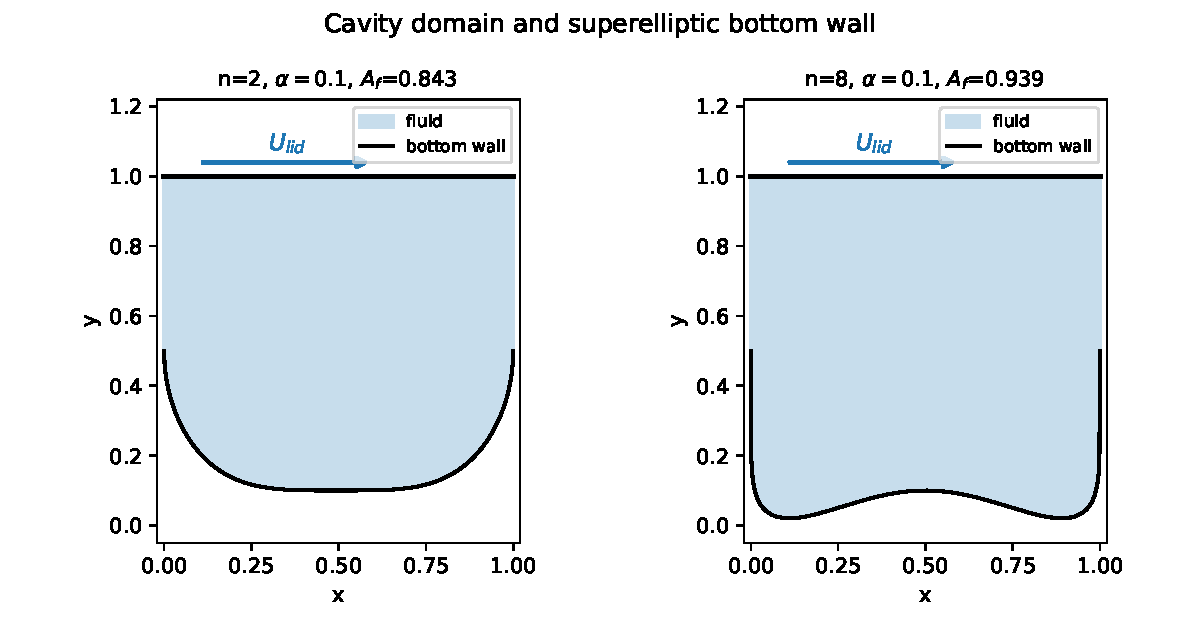
\includegraphics[width=0.85\columnwidth]{figures/fig1_geometry.pdf}
\caption{(Color online) Schematic of the lid-driven cavity with controlled bottom-wall geometry. The domain is a square enclosure of width $L$ and nominal height $L$. The top wall (lid) moves with constant velocity $U_{\mathrm{lid}}$. The bottom boundary follows a superelliptic profile with exponent $n$ and relative undulation amplitude $\alpha = h/L$. The fluid area is $A_f$ (shaded). The three bottom shapes illustrate $n=2$, $n=4$, and $n=8$ at $\alpha=0.1$; the corresponding $\alpha=0$ cases have $\alpha=0$ and are omitted here for clarity.}
\label{fig:geometry}
\end{figure}

\begin{table}[t]
\centering
\caption{Configuration matrix. The bottom wall follows the superelliptic profile of Eq.~\eqref{eq:yb}. The fluid area $A_f$ increases with $n$ toward the square-cavity value $A_f=1$.}
\label{tab:geometry}
\begin{tabular}{@{}ll@{}}
\hline
Parameter & Values \\
\hline
Reynolds number, $Re$ & $100$, $400$, $1000$ \\
Superellipse exponent, $n$ & $2$, $4$, $6$, $8$ \\
Relative undulation amplitude, $\alpha$ & $0$, $0.1$ \\
Grid resolution, $N$ & $128$, $256$, $384$ \\
Number of undulations, $N_w$ & $1$ \\
Semi-axes, $a=b$ & $0.5$ \\
Nominal cavity height, $H$ & $1$ \\
Lid velocity, $U_{\mathrm{lid}}$ & $1$ (unit) \\
\hline
Fluid area, $A_f$ ($\alpha=0$) & $0.8927$ ($n{=}2$), $0.9635$ ($n{=}4$), $0.9819$ ($n{=}6$), $0.9892$ ($n{=}8$) \\
Fluid area, $A_f$ ($\alpha=0.1$) & $0.8427$ ($n{=}2$), $0.9135$ ($n{=}4$), $0.9319$ ($n{=}6$), $0.9392$ ($n{=}8$) \\
\hline
\end{tabular}
\end{table}


\subsection{Governing equations and dimensionless groups}
\label{subsec:governing}

The flow is governed by the incompressible Navier--Stokes equations. In dimensionless form, with lengths scaled by $L$, velocities by $U_{\mathrm{lid}}$, and time by $L/U_{\mathrm{lid}}$, these read
\begin{equation}
\frac{\partial \mathbf{u}}{\partial t} + \mathbf{u}\cdot\nabla\mathbf{u} = -\nabla p + \frac{1}{Re}\nabla^2\mathbf{u}, \qquad \nabla\cdot\mathbf{u}=0,
\label{eq:NS}
\end{equation}
where the Reynolds number is $Re = U_{\mathrm{lid}} L/\nu$ and $\nu$ is the kinematic viscosity. The LBM models this incompressible system at low Mach number; the lattice Mach number $Ma = U/c_s$ (with $c_s$ the lattice sound speed) is $0.06$ or below on the production grid, but rises to about $0.09$ at $N=256$ and $0.18$ at $N=128$ for the higher Reynolds numbers because the lattice speed follows a diffusive scaling (Section~\ref{sec:numerical}). Compressibility effects are therefore small at the resolutions that support the final results but not negligible on the coarse grids, which is one reason those grids are used only for the resolution test.

\subsection{Boundary conditions}
\label{subsec:bc}

The moving lid is prescribed with a regularized velocity profile: the lid velocity is constant across the bulk of the top wall and is smoothed near the two top corners using a smoothstep with transition parameter $\varepsilon=0.02$, reducing the singularity at the corners. The side walls and the curved bottom wall satisfy the no-slip condition via interpolated bounce-back, described in Section~\ref{sec:numerical}. The distinction between physical boundary conditions and their discrete lattice realization is discussed separately below.

\subsection{Energetic measures}
\label{subsec:energetics}

Three volume-integrated quantities are computed for every converged run.

\paragraph{Power input.}
The mechanical power supplied by the moving lid is
\begin{equation}
P = \int_{\Gamma_{\mathrm{lid}}} \mathbf{u}_w \cdot (\boldsymbol{\sigma}\cdot\mathbf{n})\, dS,
\end{equation}
where $\boldsymbol{\sigma}$ is the stress tensor, $\mathbf{n}$ the outward normal, and $\mathbf{u}_w$ the lid velocity. In the LBM implementation, $P$ is extracted directly from the momentum exchange at the lid links, which corresponds to the discrete counterpart of this integral.

\paragraph{Viscous dissipation.}
For a Newtonian incompressible fluid, the total viscous dissipation is
\begin{equation}
D = 2\mu \int_{\Omega} \mathbf{S}:\mathbf{S}\, d\Omega, \qquad
\mathbf{S} = \tfrac{1}{2}\left(\nabla\mathbf{u} + (\nabla\mathbf{u})^{\mathsf{T}}\right),
\end{equation}
with $\mu$ the dynamic viscosity and $\Omega$ the fluid domain. The velocity gradients are computed from the lattice distribution functions using central differences on the grid. The domain is two-dimensional with unit depth.

\paragraph{Kinetic energy.}
The volume-integrated kinetic energy is
\begin{equation}
K = \frac{1}{2}\int_{\Omega} |\mathbf{u}|^2\, d\Omega.
\end{equation}

All three quantities are reported in dimensionless form ($P^*,D^*,K^*$) using the scaling defined in Section~\ref{sec:numerical}. The dimensionless groups are formed from $U_{\mathrm{lid}}$ and $L$ as reference scales.

\paragraph{Independence of the energetic measures.}
For the steady incompressible flow considered here, the kinetic energy is constant in time, so the global mechanical energy balance requires the power input to equal the viscous dissipation, $P=D$. The two quantities $P$ and $D$ are therefore \emph{not} independent observables: they are two discrete estimators of the same physical quantity, and the small residual $|P^*-D^*|/D^*$ reported in Section~\ref{sec:results} (a signed defect that is negative in every case and decays as a first-order-in-$1/N$ discretisation error) measures the difference between the two estimators rather than a physical energy imbalance. Consequently, the only genuinely independent second observable besides the dissipation is the kinetic energy $K^*$; the contrast $I_D$ and the power-based contrast $I_P$ are two routes to the same geometric response, and their agreement (Section~\ref{subsec:consistency}) is a consistency check, not an independent confirmation of a distinct effect. This is why the analysis is built on $I_D$ and uses $I_P$ only as a cross-check.

\subsection{Matched geometric contrasts}
\label{subsec:contrasts}

Let $q$ denote the geometric exponent, taking values $q=2,4,6,8$. For any energetic quantity $Q^*$, the matched contrast between two exponents is defined with a fixed sign convention:
\begin{equation}
I_Q(q_i,q_j) = Q^*(q_j) - Q^*(q_i), \qquad i<j.
\label{eq:contrast}
\end{equation}
The three contrasts studied are $I_Q(2,4)$, $I_Q(4,6)$, and $I_Q(6,8)$. A positive $I_D$ means that the higher-exponent geometry dissipates more energy than the lower-exponent one, under this convention. These contrasts are \emph{differences} between paired simulations, not absolute power or dissipation values; a large relative variation of a small absolute contrast must be interpreted with care, as discussed in Section~\ref{sec:results}.

Note that the estimator discrepancy $\delta_{IP/ID}$ of Section~\ref{subsec:consistency} measures the agreement between two discrete estimators of the same physical quantity; it is distinct from, and must not be confused with, the resolution uncertainty of $I_D$ itself, which is quantified in Section~\ref{subsec:robustness}.

Unless stated otherwise, contrasts are quoted as percentages of the earlier configuration of the pair,
\begin{equation}
I_Q(q_i,q_j)=\frac{Q^*(q_j)-Q^*(q_i)}{Q^*(q_i)}\times 100\%,
\end{equation}
so that the denominator is always $D^*(q_i)$ or $P^*(q_i)$ and the sign follows the numerator.

\subsection{Area-based reference model}
\label{subsec:area}

The fluid area is \emph{not} constant across the exponent transitions: increasing $n$ flattens the bottom wall toward the square-cavity limit $A_f=1$ (Table~\ref{tab:geometry}). A null hypothesis is therefore tested: that the change in dissipation across a geometric transition is fully explained by the change in fluid area, i.e.\ that the dissipation is extensive in the fluid amount. Under this hypothesis the dissipation would scale with $A_f$, and the predicted contrast would be
\begin{equation}
I_{D,\mathrm{area}}(q_i,q_j) = \left(\frac{A_f(q_j)}{A_f(q_i)} - 1\right)\times 100\%.
\label{eq:area}
\end{equation}
Since $A_f$ increases from $0.8927$ ($n=2$) to $0.9635$ ($n=4$), this extensive reference predicts a contrast of $+7.93\%$ for the transition $(2,4)$. The comparison with the measured $I_D$ in Section~\ref{subsec:arearesult} quantifies how far the actual response is from this extensive limit.
\subsection{Non-additivity and interaction}
\label{subsec:interaction}

If an interaction between the superellipse exponent and the undulation amplitude is to be claimed, it must be defined as a difference of differences, not inferred from a fitted model. For amplitude values $\alpha_1$ and $\alpha_0$,
\begin{equation}
\mathcal{I}_Q = \left[Q^*(q_j,\alpha_1)-Q^*(q_i,\alpha_1)\right] - \left[Q^*(q_j,\alpha_0)-Q^*(q_i,\alpha_0)\right].
\end{equation}
This quantity is reported when both amplitude values are available; otherwise, the discussion is restricted to the matched contrasts at fixed amplitude. With only two amplitude levels ($\alpha\in\{0,0.1\}$), $\mathcal{I}_Q$ is a single finite difference and cannot by itself establish a functional dependence on $\alpha$; it establishes only that the contrast \emph{changes} with amplitude. We therefore use $\mathcal{I}_Q$ strictly as a difference-of-differences estimator and refrain from any statement about the form of an interaction law.





\section{Numerical method and verification}
\label{sec:numerical}

\subsection{MRT-lattice Boltzmann scheme}
\label{subsec:mrt}

The solver employs a D2Q9 multiple-relaxation-time lattice Boltzmann method. The distribution functions $f_i$ are discretized on a nine-velocity square lattice. In the MRT formulation, the populations are transformed to the moment space, collided with a diagonal relaxation matrix, and transformed back before streaming. The relaxation time $\tau$ is related to the kinematic viscosity through
\begin{equation}
\nu = c_s^2\left(\tau - \tfrac{1}{2}\right)\Delta t,
\end{equation}
where $c_s^2 = 1/3$ for the D2Q9 lattice. The relaxation rates for the non-hydrodynamic moments are chosen following standard MRT practice to enhance numerical stability; only the shear mode uses $\tau$, while the remaining rates are fixed at values appropriate for the low-Mach regime considered here.

The lattice velocity is set from $U=(\tau-\tfrac12)\,Re/(3N)$, so that the target Reynolds number fixes $\tau$ through $Re=UN/\nu_{\mathrm{lat}}$ with $\nu_{\mathrm{lat}}=\tfrac13(\tau-\tfrac12)$. Table~\ref{tab:params} lists the actual $(\tau,U,Ma)$ values for each $Re$ family; the lattice Mach number is not identical across the three Reynolds numbers because $\tau$ is chosen for numerical stability rather than to keep $Ma$ fixed.

\subsection{Wall treatments}
\label{subsec:walls}

\paragraph{Curved bottom wall.}
The bottom boundary combines a staircase solid/fluid mask with Bouzidi interpolated bounce-back~\cite{Bouzidi2001}. The staircase mask classifies a cell as fluid or solid according to whether its centre lies above or below the wall $y_b(x)$, and is used only to decide which nodes are active. The boundary condition itself is not staircase: for every fluid node adjacent to the wall, the lattice link that crosses $y_b(x)$ is intersected analytically and the fractional distance $q$ to the wall is computed; the unknown population is then reconstructed by linear interpolation between the wall and the upstream fluid node, weighted by $q$. This is the standard second-order Bouzidi scheme. The distinction matters for interpretation: the mask defines the active-node set and therefore introduces a grid-dependent representation of the computational domain, whereas the Bouzidi interpolation imposes the no-slip condition at the analytic wall location. The dissipation is evaluated as a volume integral of discrete strain-rate values; its sensitivity to the near-wall gradient treatment is assessed separately in Section~\ref{subsec:robustness}.

\paragraph{Moving lid.}
The lid velocity is imposed using a regularized momentum injection: the top-wall links receive a prescribed momentum consistent with the lid velocity, smoothed near the corners with a smoothstep profile of width $\varepsilon=0.02$. This is not a Zou--He boundary nor a general regularization of the LBM collision operator; it is a link-based momentum forcing that reproduces the prescribed lid velocity while mitigating the corner singularity.

\subsection{Numerical parameter matrix}
\label{subsec:params}

The lattice velocity is set from $U=(\tau-\tfrac12)\,Re/(3N)$, i.e.\ by \emph{diffusive scaling}: $\tau$ (hence $\nu_{\rm lat}$) is fixed per Reynolds number while $U\propto1/N$, so $Ma=U/c_s$ decreases with refinement. Table~\ref{tab:params} lists the actual $(\tau,U,Ma)$ values. At $N=384$ (the production grid) $Ma\simeq0.0226$ ($Re=100$) and $Ma\simeq0.0601$ ($Re=400,1000$); at the coarser test grids the Mach number is larger---$Ma\simeq0.0338$ and $0.0902$ at $N=256$, and $Ma\simeq0.0677$ and $0.1804$ at $N=128$, for $Re=100$ and $Re\ge400$ respectively. Because the resolution study holds $\tau$ fixed at each $Re$, the grid is refined at constant physical viscosity and the comparison legitimately isolates the discretisation; the accompanying change of $Ma$ is a consequence of the diffusive scaling rather than an independent parameter. The study is nevertheless not matched in $Ma$ across Reynolds numbers, and compressibility differences between $Re=100$ and the higher Reynolds numbers are not isolated; the comparison of geometric contrasts remains internal to each Reynolds number, where $Ma$ is fixed. In addition, the fine 19-point Reynolds sweep at $N=128$ ($Re\in[100,1000]$ in steps of $50$) is fully documented in Table~SM.III of the Supplemental Material; for $Re\ge 150$ it maintains $U=5/48\approx0.104167$ ($Ma\approx0.1804$) with $\tau=0.5+40/Re$.

\begin{table}[t]
\centering
\caption{LBM numerical parameters for the three Reynolds-number families at $N=384$. $N$ is the grid resolution, $\tau$ the relaxation time, $U$ the lattice lid velocity, and $Ma=U/c_s$ the lattice Mach number.}
\label{tab:params}
\begin{tabular}{@{}ccccc@{}}
\hline
$Re$ & $N$ & $\tau$ & $U$ & $Ma$ \\
\hline
$100$  & $384$ & $0.65$ & $0.01302$ & $0.0226$ \\
$400$  & $384$ & $0.60$ & $0.03472$ & $0.0601$ \\
$1000$ & $384$ & $0.54$ & $0.03472$ & $0.0601$ \\
\hline
\end{tabular}
\end{table}
\subsection{Convergence criterion}
\label{subsec:convergence}

Each simulation is run until the relative change of the velocity field between successive measurement windows falls below $10^{-8}$. The final iteration count and residual are recorded for every case; all $24$ cases in the $N=384$ main campaign ($N_w=1$, $\alpha\in\{0,0.1\}$) satisfied this criterion, with residuals at or below $9.9\times10^{-9}$. The six supplementary cases extended to $N=512$ ($Re=400$ and $Re=1000$, $n\in\{2,4,6,8\}$, $\alpha=0$) likewise converged, with residuals between $9.86\times10^{-9}$ and $9.98\times10^{-9}$ and iteration counts between $500\,000$ and $1\,202\,000$. Iterative convergence of the discrete solution does not, by itself, establish spatial convergence of the energetic integrals; this distinction is developed in Section~\ref{subsec:resolution}.

\subsection{Numerical verification against the square-cavity benchmark}
\label{subsec:validation}

The square cavity ($A_f=1$, flat bottom) is the standard benchmark of Ghia et al.~\cite{Ghia1982}. Four verifications are reported. First, an \emph{exact} square cavity with a flat bottom and a uniform (non-regularized) lid is run directly at $Re=100$, $400$, and $1000$; the centerline profiles are compared pointwise with the tabulated data of Ghia et al.~\cite{Ghia1982} in Table~\ref{tab:ghia}. Both the horizontal velocity $u$ along the vertical centerline $x=0.5$ and the vertical velocity $v$ along the horizontal centerline $y=0.5$ match the reference to within a few percent of the lid velocity: at $N=256$ the maximum absolute deviations are $0.0062$ and $0.0102$ at $Re=100$, $0.0033$ and $0.0058$ at $Re=400$, and $0.0050$ and $0.0136$ at $Re=1000$ (the latter spectral reference case is that of Botella and Peyret~\cite{Botella1998}). The vertical-velocity error at $Re=400$ is dominated by a single non-monotone tabulated datum at $x=0.9063$ that is commonly treated as anomalous~\cite{Chai2006}; excluding it, $\max|v-v_G|$ is $0.0058$, consistent with the other Reynolds numbers. Second, the campaign includes a near-square case ($n=8$, $\alpha=0$, $A_f=0.9892<1$) that uses the \emph{regularized} production lid, compared with the same benchmark in Fig.~\ref{fig:benchmark}. Using the same interior centerline stations and the same exclusion of the anomalous $Re=400$ datum, its maximum deviations at $N=256$ are $0.0038$ and $0.0054$ at $Re=100$, $0.0035$ and $0.0034$ at $Re=400$, and $0.0046$ and $0.0066$ at $Re=1000$---i.e.\ of the same order as, and in several cases smaller than, the exact-square deviations, despite the regularized lid (which differs from the uniform lid of Ghia et al.\ near the top corners) and the small rounding of the $n=8$ bottom corners. The curved-wall (Bouzidi) treatment and the near-square bottom therefore do not degrade the interior solution. The exact-square test verifies the flat-wall and uniform-lid limits of the solver; the near-square test confirms that the curved-wall treatment does not degrade the interior solution.

Third, to isolate the effect of the regularized lid itself---separately from the curvature and rounded corners of the near-square case---the flat square cavity ($A_f=1$, strictly flat bottom) was recomputed with the \emph{regularized} production lid ($\varepsilon=0.02$) at every Reynolds number and both grids, giving a complete $Re\in\{100,400,1000\}\times N\in\{128,256\}\times\{$uniform$,$regularized$\}$ matrix. The centerline deviations from Ghia et al.\ are essentially unchanged: at $N=256$ the regularized lid gives $0.0062$ and $0.0102$ ($Re=100$), $0.0033$ and $0.0058$ ($Re=400$), and $0.0052$ and $0.0135$ ($Re=1000$) for $\max|u-u_G|$ and $\max|v-v_G|$, against $0.0062/0.0102$, $0.0033/0.0058$, and $0.0050/0.0136$ for the uniform lid---a change of at most $2\times10^{-4}$ on the finest grid. The largest difference anywhere in the matrix is $5.5\times10^{-4}$ on the coarsest grid ($Re=1000$, $N=128$), and the profiles are pointwise within the same tolerance (the full matrix is tabulated in Table~SM.VI of the Supplemental Material). The corner regularization of the lid therefore does not measurably alter the interior flow on a flat geometry; it only removes the corner singularity. This addresses the possible concern that the production lid could bias the bulk solution relative to the standard benchmark.

Fourth, and most directly relevant to the energetic claims, a conforming Taylor--Hood finite-element solver (P2 velocity / P1 pressure, Picard linearisation) was used to recompute the primary contrast $I_D(2,4)$ at $Re=400$, $\alpha=0$ on the \emph{same} superelliptic geometry (identical wall function and fluid area $A_f=0.892699$) and with the \emph{same} regularized lid profile: the prescribed top-boundary velocity reproduces the production cubic-smoothstep lid regularization of width $\varepsilon=0.02$, so the two solvers share the wall geometry, the lid boundary condition, and the definitions of the energetic integrals. All finite-element energetics are evaluated \emph{natively}: the strain-rate, lid-power, and kinetic-energy integrals are taken element-wise from the finite-element velocity field, with no projection and no lattice-Boltzmann wall-gradient model. The native energy balance of the finite-element solution closes to $0.01\%$ on its finest mesh ($P^*=D^*$ to $0.01\%$, and remains within $0.22\%$ over all three FEM meshes; Table~SM.VII of the Supplemental Material), which serves as an internal check of energetic consistency. This near-exact FEM balance closure contrasts with the lattice-Boltzmann discrete calculations, where the global energy defect $|P^*-D^*|/D^*$ is of order $2\%$ on the $N=384$ production grid (reaching up to $2.17\%$, or $\approx 2.2\%$ at most over all production runs; Table~SM.XI of the Supplemental Material), stemming from the discrete resolution of the high-shear lid boundary layer. As shown below, this defect is nearly identical between paired geometries at the same resolution and therefore largely cancels in the differential contrasts ($I_P \approx I_D$). On the finest grids of each solver (FEM $nx=ny=256$, MRT-LBM $N=384$) the absolute n$=2$ levels agree to $1$--$4\%$ ($K^*$: $+1.1\%$, $D^*$: $+2.0\%$, $P^*$: $+4.1\%$), and the three contrasts agree to within $0.02$ percentage point ($I_K$: $0.019$ pt, $I_P$: $0.008$ pt, $I_D$: $0.002$ pt; Table~\ref{tab:femxcheck} and Fig.~\ref{fig:femxcheck}). The dissipation contrast is the most cleanly reproduced: the finite-element sequence $I_D(2,4)=+0.346\%$ ($nx=64$), $+0.332\%$ ($nx=128$), $+0.323\%$ ($nx=256$) is monotone and approaches the lattice-Boltzmann value $+0.325\%$ at $N=384$. The proximity on the finest grids ($0.002$ pt) is encouraging but is a consistency check, not a convergence proof: the finite-element variation across its own three meshes ($0.023$ pt, from $+0.346\%$ to $+0.323\%$) is larger than the final FEM--LBM gap, so the calculation does not by itself demonstrate that the finite-element estimate converges to the lattice-Boltzmann one. The larger absolute $P^*$ offset reflects the rougher resolution of the lid shear layer at $N=384$ together with the residual $2\%$ lattice-Boltzmann power--dissipation imbalance there; it cancels in the paired contrast, as the internal-consistency argument of Section~\ref{subsec:resolution} predicts. The finite-element cross-check therefore corroborates the contrast (to $\lesssim0.02$ pt) and, once each solver is taken at its own finest grid, the absolute dissipation (to $2\%$); it is reported as an independent-solver consistency check, not as a second convergence study. The FEM--LBM comparison is therefore reported strictly as a cross-solver consistency check at $Re = 400$, never as a convergence proof for either solver.

The same solver was run at $Re=1000$, where the check is more informative because the contrast is larger. Restricted to its native element-wise diagnostics it gives $I_D(2,4)=+0.716\%$ at $nx=64$ and $+0.598\%$ at $nx=128$, against $+0.5909\%$ on the lattice-Boltzmann production grid $N=384$: the finer mesh differs by $0.008$ percentage point, or $1.3\%$ in relative terms, and the native finite-element sequence moves toward the lattice-Boltzmann value under refinement. The LBM-grid-projected finite-element contrasts are $+32.6\%$ ($nx=64$) and $+11.8\%$ ($nx=128$) and are not used: projecting the finite-element solution onto the coarser lattice under-resolves the lid shear layer at this Reynolds number. The same projection is already unreliable at $Re=400$, where it yields $+6.1\%$ at $nx=64$ and $+2.0\%$ on the mesh used for the finest native value, against $+0.323\%$ natively. All finite-element--lattice-Boltzmann comparisons in this work therefore use native element-wise integrals.

This verification supports the correctness of the bulk fluid solver and of the curved-wall treatment. The energetic integrals are volume integrals of the stress tensor, so their resolution sensitivity is examined separately in Section~\ref{subsec:resolution}.

\begin{table}[t]
\centering
\caption{Independent-solver cross-validation of the primary contrast $(2,4)$ at $Re=400$, $\alpha=0$: Taylor--Hood finite-element method (P2/P1) \emph{vs.}\ the MRT-LBM, on the identical superelliptic geometry. The comparison is made on the finest grids of each solver (FEM $nx=ny=256$, MRT-LBM $N=384$). All FEM entries are \emph{native}: the strain-rate, lid-power, and kinetic-energy integrals are evaluated element-wise from the finite-element velocity field, without projection. The upper block gives the absolute $n=2$ reference values together with the FEM--LBM \emph{relative} difference (in percent); the lower block gives the geometric contrast $I(2,4)$, whose FEM--LBM difference is expressed in percentage points (pt). The finite-element native energy balance closes to $0.01\%$ on $nx=256$ (and within $0.22\%$ across all FEM meshes). The FEM--LBM contrast differences $\Delta$ (in pt) are computed from the unrounded solver outputs, not from the displayed three-decimal contrasts.}
\label{tab:femxcheck}
\small
\begin{tabular}{@{}lcccc@{}}
\toprule
Quantity & FEM & MRT-LBM & $\Delta_{\rm rel}$ [\%] & $\Delta$ [pt] \\
\midrule
$K^*$ ($n=2$), native  & $0.040440$ & $0.040011$ & $+1.1$ & --- \\
$P^*$ ($n=2$), native  & $23.899$   & $22.954$   & $+4.1$ & --- \\
$D^*$ ($n=2$), native  & $23.896$   & $23.432$   & $+2.0$ & --- \\
$D^*$ ($n=4$), native  & $23.973$   & $23.508$   & $+2.0$ & --- \\
\midrule
$I_{K}(2,4)$ [\%]      & $+0.752$   & $+0.771$   & --- & $0.019$ \\
$I_{P}(2,4)$ [\%]      & $+0.321$   & $+0.328$   & --- & $0.008$ \\
$I_{D}(2,4)$ [\%]      & $+0.323$   & $+0.325$   & --- & $0.002$ \\
\bottomrule
\end{tabular}
\end{table}

\begin{figure}[t]
\centering
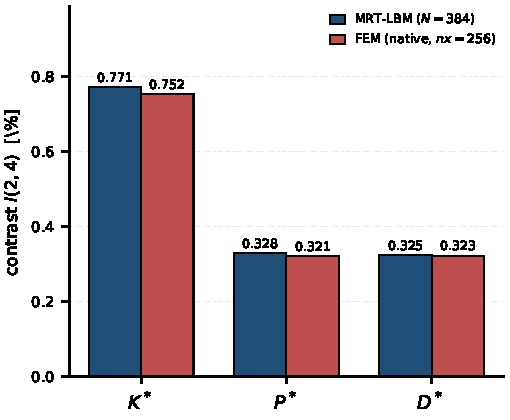
\includegraphics[width=0.75\columnwidth]{figures/fig10_fem_xcheck.pdf}
\caption{(Color online) Independent-solver cross-validation at $Re=400$, $\alpha=0$. Geometric contrast $I(2,4)$ of the kinetic energy $K^*$, lid power $P^*$, and viscous dissipation $D^*$, computed on the finest grids of each solver---MRT-LBM ($N=384$, left bars) and Taylor--Hood finite-element (native, $nx=ny=256$, right bars)---on the same superelliptic geometry. All three contrasts agree to within $0.02$ percentage point; the finite-element values use the native element-wise strain-rate, lid-power, and kinetic-energy integrals (Table~\ref{tab:femxcheck}).}
\label{fig:femxcheck}
\end{figure}

\begin{figure}[t]
\centering
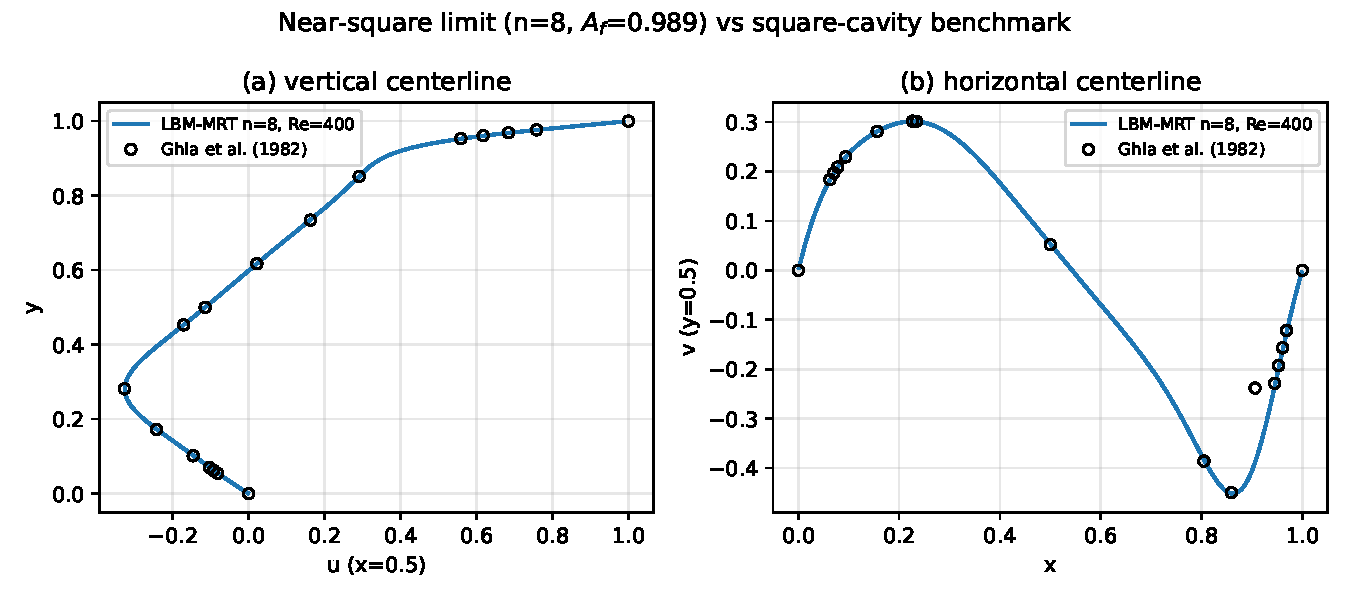
\includegraphics[width=0.9\columnwidth]{figures/fig2_benchmark.pdf}
\caption{(Color online) Near-square verification. Centerline velocity profiles of the $n=8$, $\alpha=0$ case at $Re=400$, $N=384$ (solid lines), compared with the square-cavity benchmark of Ghia et al.~\cite{Ghia1982} (open symbols). (a) Horizontal velocity $u$ along the vertical centerline $x=0.5$; (b) vertical velocity $v$ along the horizontal centerline $y=0.5$. The geometry is the closest available to the square limit ($A_f=0.9892$).}
\label{fig:benchmark}
\end{figure}

\begin{table}[t]
\centering
\caption{Exact square-cavity verification (flat bottom, uniform lid) against Ghia et al.~\cite{Ghia1982}. Maximum absolute deviations of the centerline velocity profiles at the tabulated interior reference stations: $\max|u-u_G|$ along the vertical centerline and $\max|v-v_G|$ along the horizontal centerline. The final column excludes the single anomalous tabulated datum at $(Re{=}400,\,x{=}0.9063)$~\cite{Chai2006}.}
\label{tab:ghia}
\small
\begin{tabular}{rrrrr}
\toprule
$Re$ & $N$ & $\max|u-u_G|$ & $\max|v-v_G|$ & $\max|v-v_G|$ (excl.) \\
\midrule
$100$  & $128$ & $0.0075$ & $0.0109$ & $0.0109$ \\
$100$  & $256$ & $0.0062$ & $0.0102$ & $0.0102$ \\
$400$  & $128$ & $0.0080$ & $0.1458$ & $0.0075$ \\
$400$  & $256$ & $0.0033$ & $0.1492$ & $0.0058$ \\
$1000$ & $128$ & $0.0120$ & $0.0107$ & $0.0107$ \\
$1000$ & $256$ & $0.0050$ & $0.0136$ & $0.0136$ \\
\bottomrule
\end{tabular}
\end{table}
\subsection{Resolution-sensitivity strategy}
\label{subsec:resolutionstrategy}

Three grid resolutions are employed: $N=128$, $256$, and $384$, corresponding to refinement factors of $2$ and $1.5$. These are chosen to bracket the finest resolution that can be afforded for the full parameter matrix within available compute resources, and to expose any non-monotonic behavior that a two-point comparison would miss. The refinement ratios are not uniform, and the residual change between the two finest grids is dominated by the partial cancellation of common discretization error rather than by a clean power-law decay; no Richardson extrapolation or grid-convergence index is therefore reported. Instead, the raw values at all three resolutions are reported and the span over $N=128$--$384$ is retained as a conservative numerical uncertainty (Section~\ref{subsec:robustness}). The language of ``resolution sensitivity'' is retained throughout; the term ``grid-independent solution'' is not used, since the data do not establish it to that standard.

\section{Results and discussion}
\label{sec:results}

\subsection{Overview of the campaign}
\label{subsec:overview}

The campaign comprises $24$ converged simulations at $N=384$: three Reynolds numbers ($Re=100$, $400$ and $1000$), the full exponent sequence ($n=2$, $4$, $6$ and $8$) at each of them, and the two amplitudes $\alpha=0$ and $0.1$. Additional runs at $N=128$ and $N=256$ provide the resolution-sensitivity data of Section~\ref{subsec:resolution}. All $N=384$ simulations met the iterative criterion with final relative velocity changes at or below $9.9\times10^{-9}$. The complete scalar dataset is tabulated in the supplementary material; only the cases that support the argument are discussed here.

\subsection{Representative flow fields}
\label{subsec:fields}

Figure~\ref{fig:fields} presents the velocity-magnitude streamlines at $Re=400$, $N=384$ for all eight combinations $(n,\alpha)\in\{2,4,6,8\}\times\{0,0.1\}$ on a common color scale (colorbar in Fig.~\ref{fig:fields}). Two representative levels are shown because the full exponent sequence is now available at all three Reynolds numbers and $Re=400$ is the intermediate one, and because the undulated wall ($\alpha=0.1$) clears a larger portion of the cavity than the flat one; presenting both in the same figure avoids reporting the flat-wall fields in isolation. In all eight panels the lid drives a single dominant recirculation cell whose centre stays close to the cavity centre. The undulation produces a weak secondary structure attached to the bottom trough and a slightly more distorted near-wall shear layer, whereas increasing $n$ mainly flattens the bottom contour and removes the near-corner fillet. The change from $n=2$ to $n=4$ is the largest single geometric step; for $n=6$ and $n=8$ the streamline patterns at a given amplitude become nearly indistinguishable. These images are qualitative only: the quantitative energetic response, including the amplitude interaction, is given in Figs.~\ref{fig:energetic} and~\ref{fig:contrasts}. Complete field maps for every converged configuration, again separated by amplitude, are compiled in the supplementary material (Figs.~SM.2 and SM.3).

\begin{figure}[t]
\centering
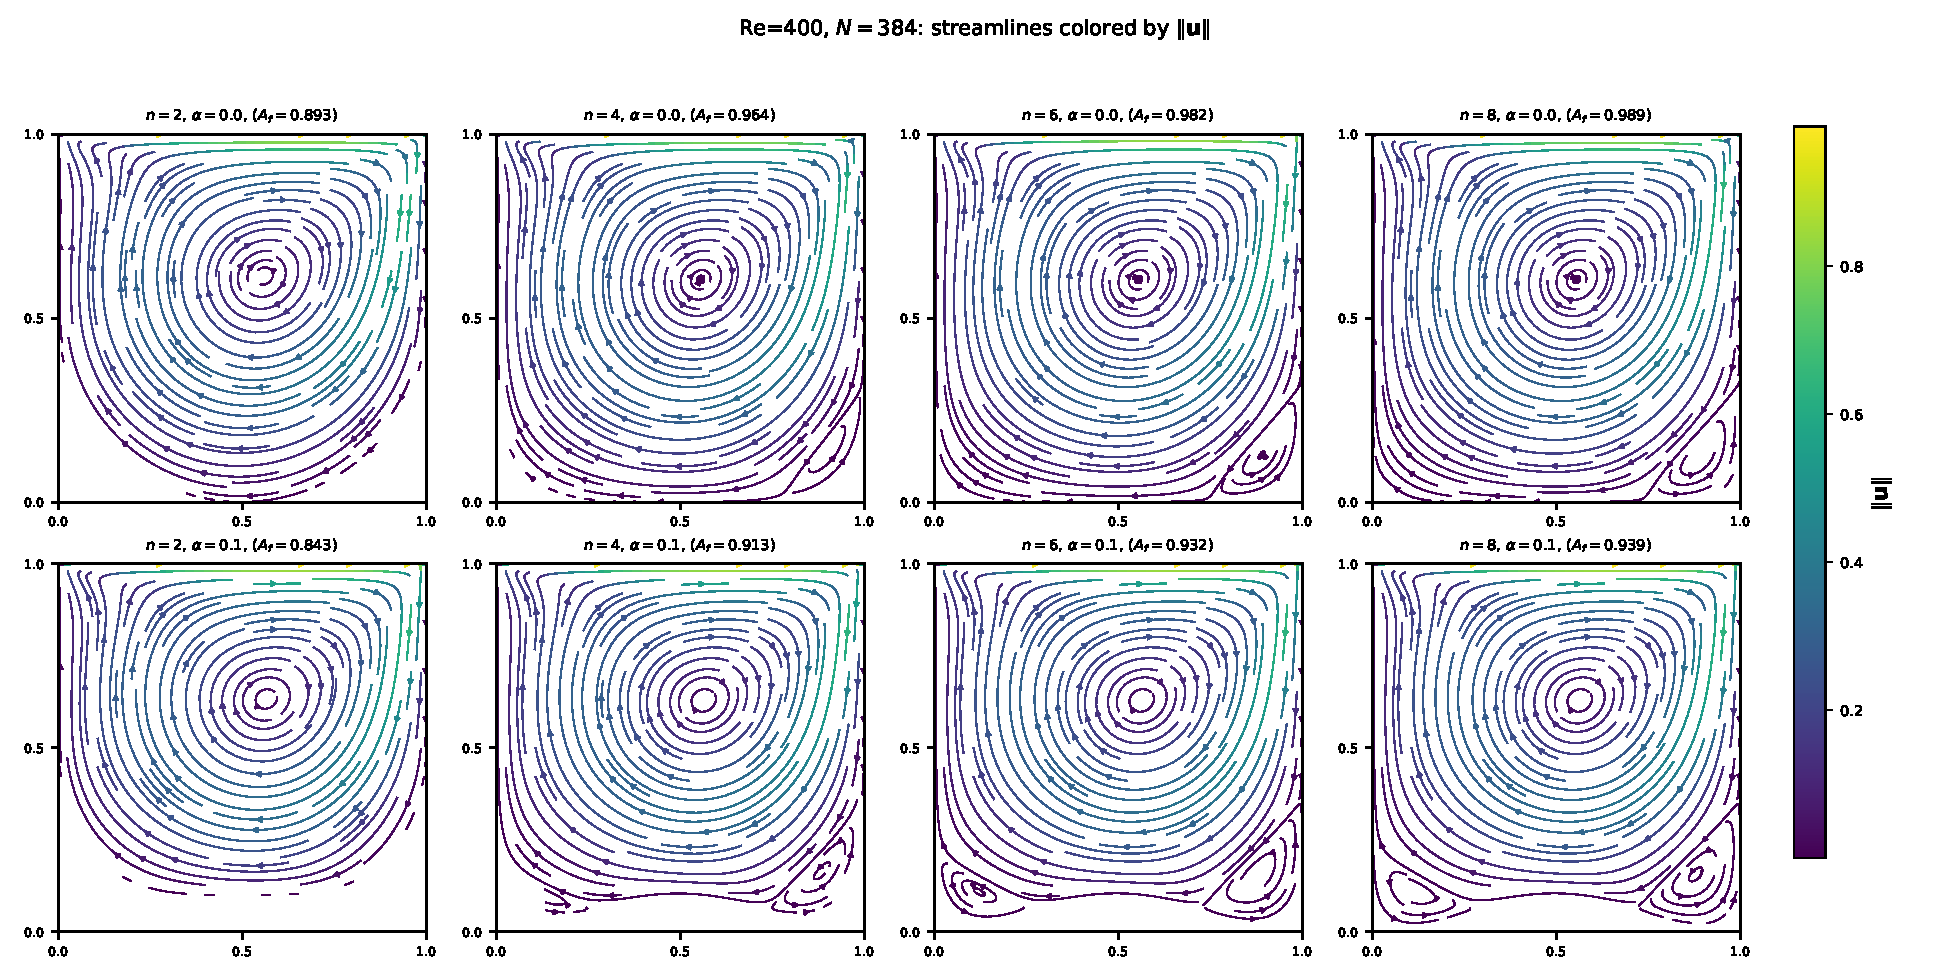
\includegraphics[width=0.98\columnwidth]{figures/fig3_fields.pdf}
\caption{(Color online) Streamlines colored by velocity magnitude at $Re=400$, $N=384$. Top row: $\alpha=0$ ($n=2$,$4$,$6$,$8$). Bottom row: $\alpha=0.1$ ($n=2$,$4$,$6$,$8$). Panels labeled by $(n,\alpha)$ with fluid area $A_f$. All panels share a common color scale $\|\mathbf{u}\|$ as indicated; the inclusion of both amplitudes allows a direct qualitative comparison between undulated and non-undulated cavities for each exponent.}
\label{fig:fields}
\end{figure}

\subsection{Spatial origin of the geometric contrast}
\label{subsec:mechanism}

The global integrals show \emph{that} the dissipation responds weakly to the bottom geometry; we now localize \emph{where} the change occurs. Figure~\ref{fig:dissipation} shows the local dissipation density $2\mu\,\mathbf{S}{:}\mathbf{S}$ at $Re=400$, $\alpha=0$, for $n=2$ and $n=4$, together with their difference $\Delta(2\mu\mathbf{S}{:}\mathbf{S})$. The dissipation is overwhelmingly concentrated in the shear layer under the lid: integrating over horizontal bands, the top $10\%$ of the cavity contains $77.8\%$ of $D^*$ at $Re=400$ and the top $20\%$ contains about $90\%$; the bottom-wall band below $y_b+0.1$ holds only $1.0\%$ ($n=2$) and $0.4\%$ ($n=4$). This near-lid concentration is nearly a one-parameter function of $Re$, and it \emph{weakens} slowly with Reynolds number---the top-$10\%$ share falls from $83.7\%$ at $Re=100$ to $77.8\%$ at $Re=400$ and $74.3\%$ at $Re=1000$---because the core circulation thickens and spreads its dissipation over a larger fraction of the cavity as $Re$ increases. The lid layer nevertheless remains the dominant dissipative zone at all three Reynolds numbers.

The geometric contrast is therefore not a bottom-wall friction effect. To localize it exactly, we partition the $n=4$ fluid region into two disjoint parts: the \emph{common} region $A$, consisting of cells that are fluid for both $n=2$ and $n=4$, and the \emph{added} region $B$, consisting of cells that are fluid for $n=4$ but solid for $n=2$ (the shoulder zones uncovered by flattening the bowl into the near-square). Then $\Delta D$ splits, cell by cell, into a redistribution term over $A$ and an added-zone term over $B$,
\begin{equation}
\Delta D \;=\; \underbrace{\sum_{A}\big(\ell_4-\ell_2\big)}_{dA}\;+\;\underbrace{\sum_{B}\ell_4}_{dB},
\end{equation}
where $\ell$ is the local dissipation density times the cell area. Because $A$ and $B$ are disjoint and their union is exactly the $n=4$ region, this identity closes to machine precision; there is no residual partition ambiguity. Table~\ref{tab:layers} reports the two terms at the three Reynolds numbers, together with their sum, which reproduces the headline contrast $I_D$ (defined in Eq.~\ref{eq:contrast}) to within $10^{-5}$ of itself.

\begin{table}[t]
\centering
\caption{Exact partition of the geometric dissipation contrast $\Delta D$ at $\alpha=0$, $N=384$. All entries are in units of $10^{-4}D^*(2,0)$. $dA$ is the redistribution within the region common to both geometries (its four disjoint bands are listed in Table~SM.XIII of the Supplementary Material); $dB$ is the dissipation of the added region available only to $n=4$. The last two columns are the sum $dA+dB=\Delta D$ and the corresponding headline contrast $I_D(2,4)=100\,\Delta D/D^*(2,0)$. The identity closes to machine precision.}
\label{tab:layers}
\begin{tabular}{@{}lcccc@{}}
\hline
$Re$ & $dA$ (common) & $dB$ (added) & $\Delta D=dA+dB$ & $I_D$ [\%] \\
\hline
$100$  & $-4.81$ & $+6.99$ & $+2.18$ & $+0.0218$ \\
$400$  & $+12.78$ & $+19.71$ & $+32.49$ & $+0.3249$ \\
$1000$ & $+10.44$ & $+48.65$ & $+59.09$ & $+0.5909$ \\
\hline
\end{tabular}
\end{table}

Two robust facts follow. First, the \emph{added} region always makes a positive contribution $dB$: uncovering the shoulder zones adds dissipation, and this term grows monotonically with Reynolds number, from $+6.99\times10^{-4}$ at $Re=100$ to $+4.87\times10^{-3}$ at $Re=1000$ (in units of $D^*(2,0)$). Crucially, the added region is weakly dissipative: it covers about $7.4\%$ of the total fluid area at $Re=400$ yet contributes only $0.20\%$ of $D^*$, so its mean dissipation density is about $2.7\%$ of the cavity average (about $1\%$ at $Re=100$ and $7\%$ at $Re=1000$). This is the most direct explanation of the sub-extensive response: the fluid added by flattening sits in a slow, weakly sheared shoulder region and dissipates almost nothing. Second, the redistribution term $dA$ is a small difference of much larger, opposing contributions from the four disjoint bands of the common region (Table~SM.XIII of the Supplementary Material): at $Re=400$ the lid band ($y>0.9$) contributes $+2.44\times10^{-3}$ and the interior core contributes $-2.83\times10^{-3}$, whose near-cancellation plus the bottom ($+6.21\times10^{-4}$) and side/corner ($+1.04\times10^{-3}$) bands leaves the small $dA=+1.28\times10^{-3}$; at $Re=1000$ the lid band is $+5.55\times10^{-3}$ and the core $-6.60\times10^{-3}$. The redistribution term $dA$ is negative only at $Re=100$ ($-4.81\times10^{-4}$) and changes sign near $Re\approx145$, as the low-$Re$ corner-dominated balance tips toward the lid-dominated one; the added-zone term $dB$ never changes sign. Note that $dA$ and $dB$ are \emph{not} of opposite sign at $Re\ge400$---both are positive---so the smallness of the net contrast is due to the near-cancellation \emph{inside} $dA$ (between the lid and core bands), not to a cancellation between $dA$ and $dB$. The mechanism is thus a competition between an always-positive but weakly dissipative added region and a common-region redistribution that is itself a near-cancellation of opposing band contributions.

The grid robustness of this mechanism is assessed in Table~SM.XV and Fig.~SM.5 of the Supplementary Material, where all four bands are recomputed cell by cell with the identical exact-partition code at every resolution $N=128$, $256$, $384$, and $512$ (the $N=384$ rows reproduce the headline partition to machine precision, and $N=512$ is available at $Re=400$ and $1000$). The cancellation index $C=\sum|\text{bands}|/|dA|$ grows both with Reynolds number and with refinement: about $4.0$ at $Re=100$, $5.0\to5.4$ at $Re=400$, and $11.3\to14.3$ at $Re=1000$ from $N=128$ to $N=512$, reflecting the increasing internal cancellation within $dA$ as the lid and core bands become larger and more opposed. Despite this, the net contrast $\Delta D = dA + dB$, which equals $I_D(2,4)$, remains stable to within $2.4\%$ of its value across $N=128$--$512$ at all three Reynolds numbers, because the grid-induced changes in $dA$ and $dB$ partially cancel. The sign and order of magnitude of $dA$ and $dB$ are therefore robust on every grid; their individual magnitudes carry a grid sensitivity that rises with $Re$ (the $dA$ span is $1.9\%$ of its value at $Re=100$, $8.2\%$ at $Re=400$ and $27\%$ at $Re=1000$), which is the price of the internal cancellation but does not contaminate the net contrast.

\begin{figure}[t]
\centering
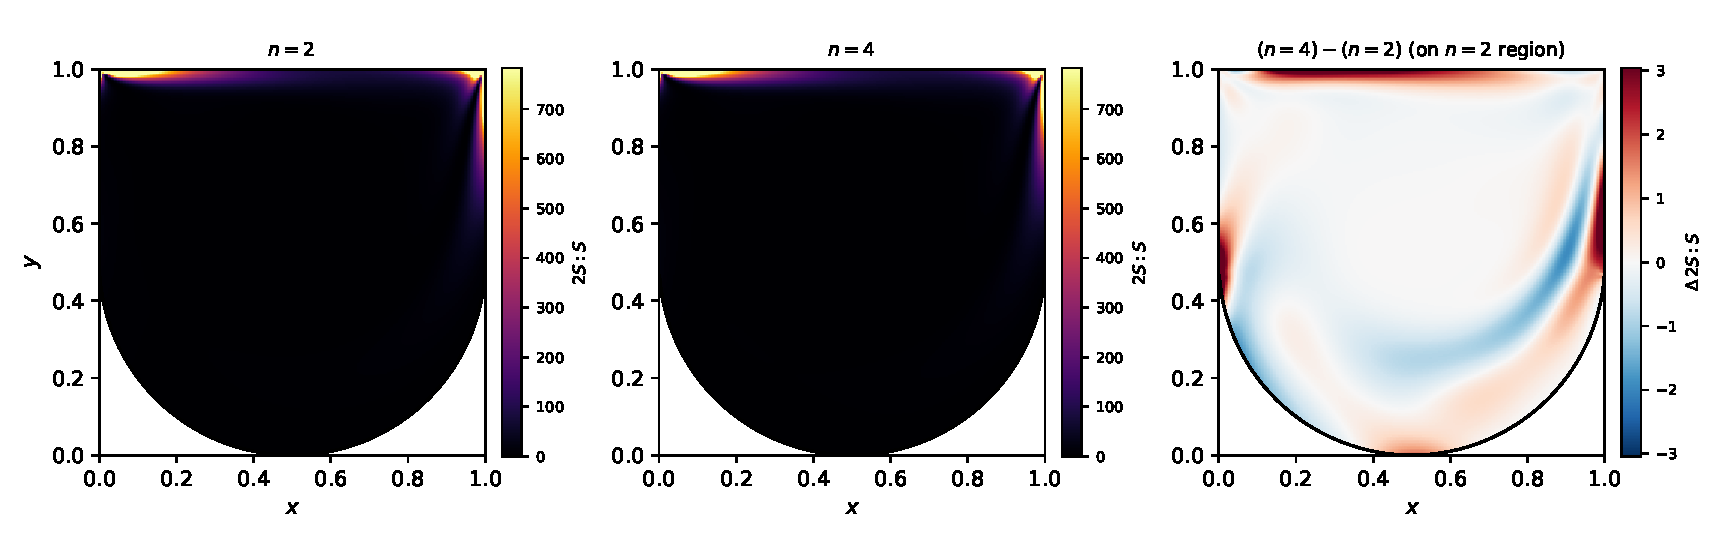
\includegraphics[width=0.98\columnwidth]{figures/fig7_dissipation_map.pdf}
\caption{(Color online) Local dissipation density $2\mu\,\mathbf{S}{:}\mathbf{S}$ at $Re=400$, $\alpha=0$, $N=384$: (left) $n=2$; (middle) $n=4$; (right) the difference $(n{=}4)-(n{=}2)$ evaluated on the $n=2$ fluid region. The dissipation is concentrated in the lid shear layer; the geometric contrast arises from a positive contribution of the added shoulder region plus a common-region redistribution that is a near-cancellation of a positive lid-band change against a negative interior-core change (Table~\ref{tab:layers}).}
\label{fig:dissipation}
\end{figure}

\subsection{Absolute energetic response}
\label{subsec:absresponse}

Figure~\ref{fig:energetic} shows $P^*$, $D^*$, and $K^*$ versus $n$ at $N=384$ for $\alpha=0$ (solid) and $\alpha=0.1$ (dashed). Several features are common to all Reynolds numbers. The power input and the dissipation increase strongly with $Re$: at $n=2$, $\alpha=0$, $D^*$ rises from $17.92$ ($Re=100$) to $23.43$ ($Re=400$) and $31.54$ ($Re=1000$). At fixed $Re$, both $P^*$ and $D^*$ increase slightly with $n$. The kinetic energy behaves differently: although it changes very little in \emph{absolute} terms over the exponent range (its total variation is below $1\%$ of its own value, and its curves in Fig.~\ref{fig:energetic} are visibly flat), its \emph{relative} geometric contrast $I_K(2,4)$ is actually larger than $I_D(2,4)$: $+0.67\%$ versus $+0.022\%$ at $Re=100$ and $+0.77\%$ versus $+0.32\%$ at $Re=400$ (at $Re=1000$ the ordering reverses, $I_K=+0.53\%$ against $I_D=+0.59\%$). The weak curvature of the $K^*$ curves therefore does not mean that $K^*$ is insensitive to the geometry: flattening the bottom shifts the recirculation slightly, and the relative change of the stored kinetic energy is comparable to, or larger than, that of the dissipation. What is genuinely small is the change of $D^*$ \emph{relative to the change in fluid area}, which is the sub-extensivity discussed next.

The small magnitude of the change in $D^*$ with $n$ is the central observation. Between $n=2$ and $n=4$ at $\alpha=0$, the fluid area grows by $7.9\%$ (from $0.8927$ to $0.9635$), yet $D^*$ grows by only $0.022\%$ ($Re=100$), $0.325\%$ ($Re=400$), and $0.591\%$ ($Re=1000$). The dissipation is therefore strongly sub-extensive relative to the area-only null model: adding fluid by flattening the bottom does not add a proportional amount of viscous dissipation, but instead reduces the dissipation per unit fluid area by approximately $7\%$ (Section~\ref{subsec:arearesult}). The remaining transitions are even weaker: at $Re=400$ the change from $n=4$ to $n=6$ adds $0.013\%$, and from $n=6$ to $n=8$ essentially nothing ($6\times10^{-5}\%$). At $Re=1000$ the same two steps are $+0.0103\%$ and $-0.0037\%$: the trailing transition is no longer vanishing but slightly negative, a point taken up in Section~\ref{subsec:contrastresult}. At $Re=100$ they are $+0.00296\%$ and $+0.00042\%$. The absolute values for all cases are collected in the supplementary material.

\begin{figure}[t]
\centering
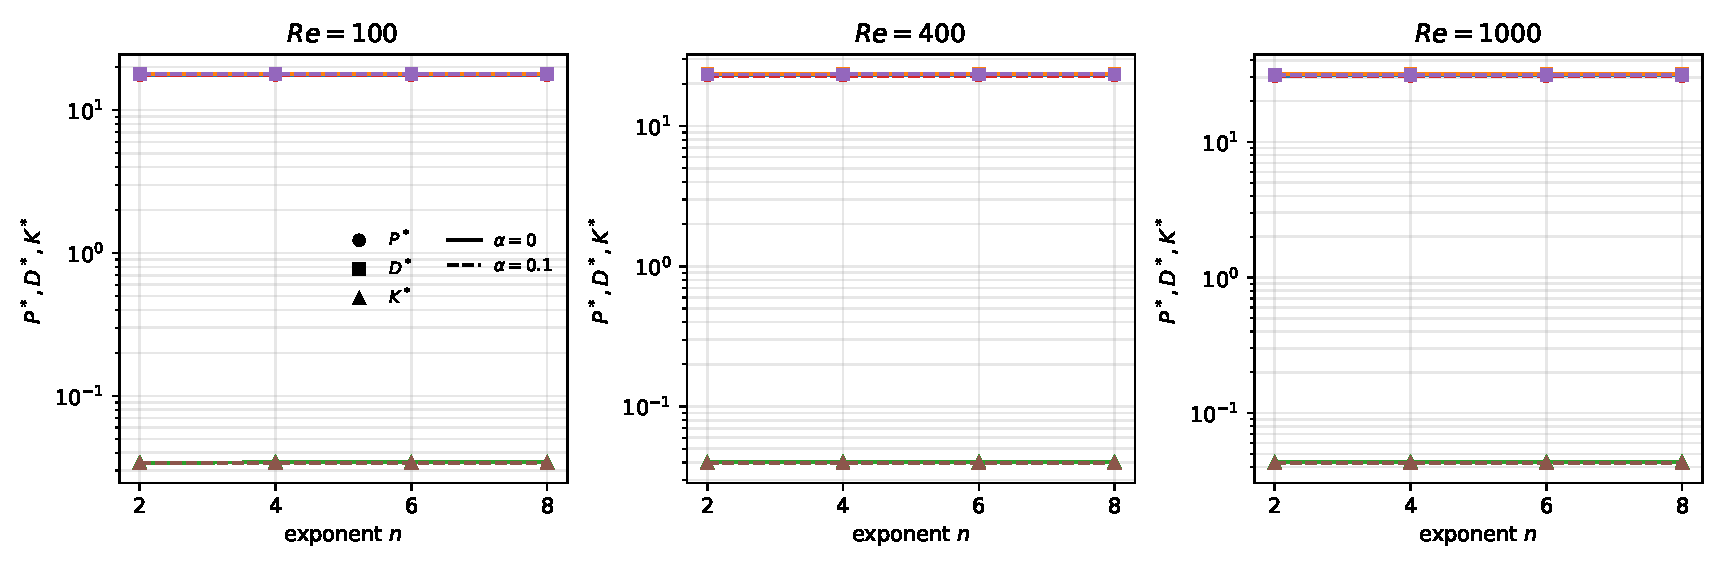
\includegraphics[width=0.95\columnwidth]{figures/fig4_energetic.pdf}
\caption{(Color online) Dimensionless energetic integrals versus superellipse exponent at $N=384$. Panels: (a) $Re=100$; (b) $Re=400$; (c) $Re=1000$. Solid lines: $\alpha=0$; dashed lines: $\alpha=0.1$. Circles: $P^*$; squares: $D^*$; triangles: $K^*$. The full sequence $n=2,4,6,8$ is available at all three Reynolds numbers. $P^*$ and $D^*$ vary strongly with $Re$ and weakly with $n$; $K^*$ is almost insensitive to $n$.}
\label{fig:energetic}
\end{figure}

\subsection{Test of the area-only extensive reference}
\label{subsec:arearesult}

Because $A_f$ increases with $n$, the extensive area reference of Eq.~\eqref{eq:area} is not identically zero. Figure~\ref{fig:contrasts} compares the measured contrasts $I_D$ and $I_P$ with $I_{D,\mathrm{area}}$ on a symmetric logarithmic ordinate: panel (a) resolves the three successive transitions at $Re=400$, and panel (b) the primary transition at the three Reynolds numbers. For the transition $(2,4)$ at $\alpha=0$, the extensive reference predicts $+7.93\%$, whereas the measured $I_D$ is $+0.022\%$ ($Re=100$), $+0.325\%$ ($Re=400$), and $+0.591\%$ ($Re=1000$). The measured and predicted contrasts share the same sign but differ in magnitude by factors of about $360$, $24$, and $13$, respectively. For $(4,6)$ the reference predicts $+1.91\%$ against a measured $+0.013\%$ at $Re=400$; for $(6,8)$ it predicts $+0.75\%$ against a measured $+6\times10^{-5}\%$ for $I_D$, while the power-based value is slightly negative ($I_P=-1.5\times10^{-4}\%$). 

The area-only model therefore does not explain the observations: it over-predicts the contrast, by factors of approximately $13$--$364$ across the Reynolds numbers studied. The correct reading is not that area is irrelevant---the area does change, and the dissipation does increase with $n$---but that the flow reorganizes so that the dissipation per unit fluid area decreases as the cavity is flattened. The area-only model is thus a simple extensive reference, not a quantitative prediction of the energetic response.

A sharper reference is the dissipation \emph{per unit fluid area}, $d^*=D^*/A_f$, which removes the trivial extensive part of the geometric change. At the primary transition this intrinsic density contrast, $I_{D/A}=100\,(d^*_4-d^*_2)/d^*_2$, is $-7.33\%$ ($Re=100$), $-7.05\%$ ($Re=400$), and $-6.80\%$ ($Re=1000$)---almost constant in $Re$ and strikingly close to the area-only prediction of $+7.93\%$ with the opposite sign. The area-only model sets the \emph{extensive} scale of the change; measured against that scale, the flow converts the added fluid into a proportionally \emph{lower} average dissipation rate. The per-area reference is therefore the physically meaningful baseline: it is $O(1)$ where the extensive reference over-predicts by factors of $13$--$364$. It should be read as a change of normalization rather than as an independent physical observable: when $I_D$ is small, $I_{D/A}$ is algebraically close to $-I_{D,\mathrm{area}}$, so its near-constant value of about $-7\%$ reflects the smallness of $I_D$ itself, not a separate physical mechanism. The physically independent information about the mechanism is carried by the $\mathrm{d}A/\mathrm{d}B$ partition of Section~\ref{subsec:mechanism} and Table~\ref{tab:layers}, not by the per-area normalization. The resolution-sensitivity analysis of Section~\ref{subsec:resolution} shows, however, that the per-area contrast inherits the residual grid error of the absolute area (the discrete mask area differs from the analytic area by at most $\sim0.02\%$ at $N=384$; see the area table of the supplementary material); we therefore quote both the extensive and per-area references and base no conclusion on their difference. Figure~\ref{fig:reference} summarizes the comparison.

\subsection{Matched geometric contrasts and their hierarchy}
\label{subsec:contrastresult}

Figure~\ref{fig:contrasts} and Table~\ref{tab:contrasts} summarize the successive contrasts. At $Re=400$, $\alpha=0$, the three measured dissipation contrasts are $I_D(2,4)=+0.3249\%$, $I_D(4,6)=+0.0129\%$, and $I_D(6,8)=+6\times10^{-5}\%$. The $(6,8)$ value is at or below its own $N = 128$--$384$ span ($1.1\times10^{-4}$~pp) and is quoted only as an upper bound; it is not resolved. Their shares of the sum of absolute magnitudes are approximately $96.2\%$, $3.8\%$, and $0.02\%$, respectively. These percentages are shares of the sum of the absolute magnitudes of the three successive contrasts; they are not fractions of a total energy budget. The same three-step sequence is now available at all three Reynolds numbers: $+0.0218\%$, $+0.00296\%$, $+0.00042\%$ at $Re=100$ and $+0.5909\%$, $+0.0103\%$, $-0.0037\%$ at $Re=1000$, i.e.\ shares of $86.6\%$, $11.8\%$, $1.7\%$ at $Re=100$ and $97.7\%$, $1.7\%$, $0.6\%$ at $Re=1000$. The concentration of the response in the $(2,4)$ transition is thus found at every Reynolds number studied, at very different absolute magnitudes.

At all three Reynolds numbers, for which the full exponent sequence is now available, the hierarchy $|I(2,4)|\gg|I(4,6)|\gg|I(6,8)|$ holds at both amplitudes examined (Section~\ref{subsec:amplitude}). It reflects the fact that the largest geometric change occurs at low $n$: the relief flattens most rapidly between $n=2$ and $n=4$, after which the cavity is already close to the square limit and further increases of $n$ alter the geometry only weakly. This is a statement about the range of exponents studied; it does not define a universal threshold at $n=4$ for other wall shapes or undulation counts.

At $Re=1000$, however, the trailing transitions do not vanish: $I_D(6,8)=-0.0037\%$ at $\alpha=0$, so beyond $n=4$ increasing the exponent slightly \emph{reduces} dissipation at the highest Reynolds number. This negative sign is resolved rather than marginal. The contrast is negative on all three grids ($-0.00371\%$, $-0.00360\%$, $-0.00371\%$ at $N=128$, $256$, $384$), with a span of $1.1\times10^{-4}$ percentage points, i.e.\ more than thirty times smaller than its own magnitude, and $(4,6)=+0.0103\%$ is likewise resolved by its own span of $4.1\times10^{-4}$ percentage points. At $Re=400$ the same $(6,8)$ transition changes sign between $N=128$ and $N=256$ and stays inside its span, so no sign can be assigned there. The $Re=1000$ value is therefore reported as the first resolved negative trailing step, not as a measured reversal from a demonstrated positive one. The undulation amplitude lowers the Reynolds number at which the trailing steps become negative: at $\alpha=0.1$ both are negative and already resolved at $Re=400$ ($-0.0039\%$ with a span of $8.7\times10^{-4}$~pp, and $-0.0017\%$ with a span of $8.5\times10^{-5}$~pp), and both stay negative at $Re=1000$ ($-0.0242\%$ and $-0.0052\%$). At $Re=100$ and $\alpha=0$ both trailing steps remain positive ($+0.00296\%$ and $+0.00042\%$); $(6,8)$ is stable across the three grids (span $8.1\times10^{-5}$~pp), whereas $(4,6)$ is not resolved at this Reynolds number, its $N=128$--$384$ span reaching $1.15$~pp because the coarse-grid $n\ge6$ cases reach a local Mach number of $0.18$ and their absolute dissipation is not comparable to the $n=4$ one there.

\begin{table}[t]
\centering
\caption{Matched dissipation and power contrasts at $N=384$, $\alpha=0$, expressed as percentages of the earlier configuration of each pair. The last three columns give the estimator discrepancy $\delta_{IP/ID}=100|I_P/I_D-1|$, the area-only extensive prediction, Eq.~\eqref{eq:area}, and the numerical uncertainty. Uncertainty is the span of the contrast itself over $N = 128$--$384$ at fixed ($Re$, transition). A contrast is treated as resolved when its magnitude exceeds its own span: this holds for every $(2,4)$ entry, for $(4,6)$ at $Re=400$ and $Re=1000$, and for $(6,8)$ at $Re=100$ and $Re=1000$, and fails for $(4,6)$ at $Re=100$ and $(6,8)$ at $Re=400$, which are therefore reported as upper bounds only (marked $\dagger$).}
\label{tab:contrasts}
\begin{tabular}{@{}ccccccc@{}}
\hline
$Re$ & Transition & $I_D$ [\%] & $I_P$ [\%] & $\delta_{IP/ID}$ [\%] & $I_{D,\mathrm{area}}$ [\%] & uncertainty [pp] \\
\hline
$100$  & $(2,4)$ & $+0.0218$ & $+0.0211$ & $3.1$  & $+7.93$ & $3.4\times 10^{-4}$ \\
$100$  & $(4,6)$ & $+0.00296$ & $+0.00264$ & $10.6$ & $+1.91$ & $1.15^{\dagger}$ \\
$100$  & $(6,8)$ & $+0.00042$ & $+0.00040$ & $4.5$  & $+0.75$ & $8.1\times 10^{-5}$ \\
$400$  & $(2,4)$ & $+0.3249$ & $+0.3282$ & $1.0$  & $+7.93$ & $2.4\times 10^{-3}$ \\
$400$  & $(4,6)$ & $+0.0129$ & $+0.0115$ & $10.3$ & $+1.91$ & $5.0\times 10^{-4}$ \\
$400$  & $(6,8)$ & $+0.00006$& $-0.00015$& --     & $+0.75$ & $1.1\times 10^{-4}$\,$^{\dagger}$ \\
$1000$ & $(2,4)$ & $+0.5909$ & $+0.6022$ & $1.9$  & $+7.93$ & $1.3\times 10^{-2}$ \\
$1000$ & $(4,6)$ & $+0.0103$ & $+0.0062$ & $40.4$ & $+1.91$ & $4.1\times 10^{-4}$ \\
$1000$ & $(6,8)$ & $-0.0037$ & $-0.0043$ & $15.6$ & $+0.75$ & $1.1\times 10^{-4}$ \\
\hline
\end{tabular}
\end{table}
\begin{figure}[t]
\centering
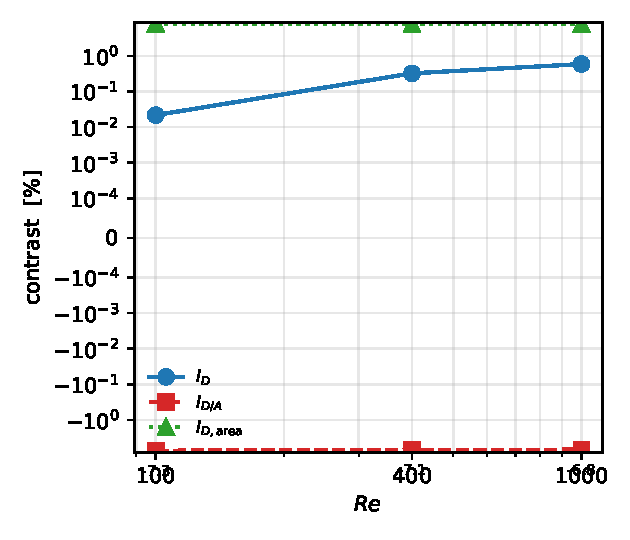
\includegraphics[width=0.6\columnwidth]{figures/fig8_reference.pdf}
\caption{(Color online) Primary transition $(2,4)$, $\alpha=0$, at $N=384$: measured dissipation contrast $I_D$ (circles), intrinsic contrast per unit fluid area $I_{D/A}$ (squares), and the extensive area-only reference $I_{D,\mathrm{area}}$ (triangles), on a symmetric logarithmic ordinate. The extensive reference lies a factor of about $24$ above the measurement, whereas the per-area contrast is the same order of magnitude with the opposite sign. The per-area curve is shown as a change of normalization, not as independent physical evidence; for small $I_D$ it is algebraically close to $-I_{D,\mathrm{area}}$.}
\label{fig:reference}
\end{figure}
\begin{figure}[t]
\centering
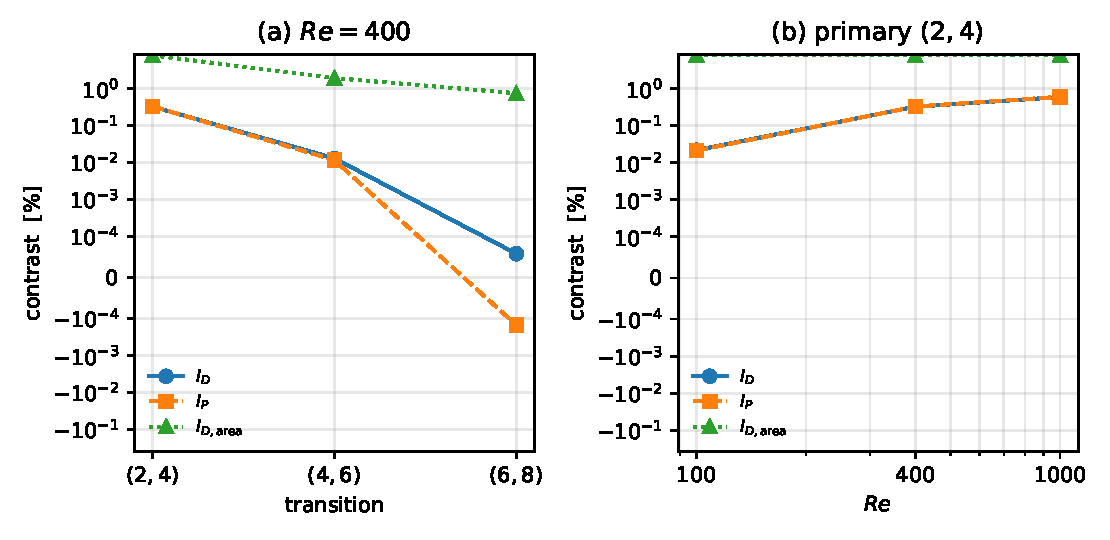
\includegraphics[width=0.95\columnwidth]{figures/fig5_contrasts.pdf}
\caption{(Color online) Matched contrasts at $N=384$, $\alpha=0$, on a symmetric logarithmic ordinate. (a) $Re=400$: the three successive transitions $(2,4)$, $(4,6)$, $(6,8)$, with dissipation $I_D$ (circles), power $I_P$ (squares), and the area-only extensive prediction $I_{D,\mathrm{area}}$ (triangles). (b) Primary transition $(2,4)$ at $Re=100$, $400$, $1000$. Every coefficient displayed has an $N=384$ value, including the slightly negative $I_P(6,8)$; no curve contains extrapolated, clipped, or missing points. The magnitude hierarchy $|I(2,4)|\gg|I(4,6)|\gg|I(6,8)|$ holds, and the measured contrasts lie below the extensive prediction by factors of $13$--$364$. At $Re=400$ the $(6,8)$ points are at or below the $N = 128$--$384$ resolution floor and are shown as upper bounds; at $Re=1000$ the $(4,6)$ and $(6,8)$ contrasts are resolved, and $(6,8)$ is negative.}
\label{fig:contrasts}
\end{figure}

\subsection{Resolution sensitivity of the contrasts}
\label{subsec:resolution}

The primary contrast $I_D(2,4)$ at $\alpha=0$ is evaluated at $N=128$, $256$, and $384$, with the target relaxation time held fixed per Reynolds number (diffusive scaling, so $U\propto1/N$) so that the comparison isolates the grid. The values are $+0.02161$, $+0.02195$, and $+0.02178\%$ at $Re=100$; $+0.32251$, $+0.32462$, and $+0.32488\%$ at $Re=400$; and $+0.57758$, $+0.58769$, and $+0.59087\%$ at $Re=1000$. Between $N=256$ and $N=384$ the relative change is $-0.8\%$ ($Re=100$), $+0.08\%$ ($Re=400$), and $+0.54\%$ ($Re=1000$), and the sequence is monotone in $N$ at $Re=400$ and $Re=1000$. At $Re=100$ the sequence is not monotone at the fourth significant figure ($+0.02161$, $+0.02195$, $+0.02178\%$); the total span over $N=128$--$384$ is $3.4\times10^{-4}$ percentage points there, i.e.\ $1.6\%$ of the contrast, against $0.73\%$ at $Re=400$ and $2.3\%$ at $Re=1000$. These spans are the conservative numerical uncertainties quoted on $I_D(2,4)$ throughout the paper, in the abstract, and in Table~\ref{tab:contrasts}. They are upper bounds: the sequence of $I_D(2,4)$ is monotone in $N$ at $Re = 400$ and $Re = 1000$, and the non-monotonicity at $Re = 100$ is at the level of the quoted precision. The contrast is therefore stable to within a few percent of its own value over the full $N=128$--$384$ range (Fig.~\ref{fig:resolution}); the residual non-monotonicity at $Re=100$ is at the level of the quoted precision rather than a systematic grid trend, and the resolution-sensitivity assessment is given in Section~\ref{subsec:robustness}.

The absolute dissipation, by contrast, is less well converged. For $n=2$, $\alpha=0$, $D^*$ changes by $+0.79\%$ ($Re=100$), $+0.78\%$ ($Re=400$), and $+0.93\%$ ($Re=1000$) between $N=256$ and $N=384$. These changes are larger than the changes in the contrast itself, which illustrates the distinction between the convergence of absolute integrals and the stability of their differences. The contrasts are relatively insensitive to resolution because the discretization errors of the two paired simulations are largely common and cancel in the difference; the absolute values still carry a residual grid dependence of order $1\%$. No claim of grid-independent absolute energetics is made, and the language of resolution sensitivity is retained throughout.

\begin{figure}[t]
\centering
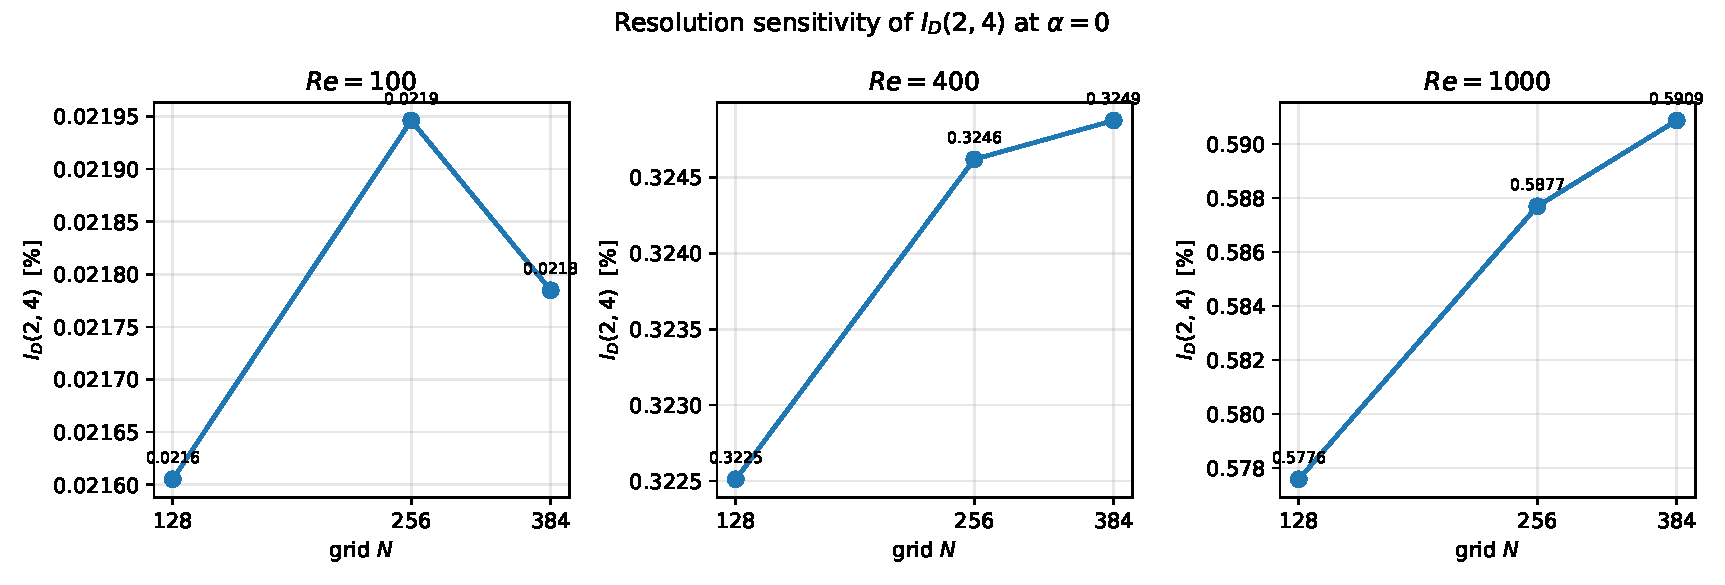
\includegraphics[width=0.95\columnwidth]{figures/fig6_resolution.pdf}
\caption{(Color online) Resolution sensitivity of the primary contrast $I_D(2,4)$ at $\alpha=0$. Panels: (a) $Re=100$; (b) $Re=400$; (c) $Re=1000$. The contrast is stable to better than $1\%$ between $N=256$ and $N=384$ at all Reynolds numbers; the full $N = 128$--$384$ spans quoted in the text are the conservative numerical uncertainties on $I_D(2,4)$ used throughout.}
\label{fig:resolution}
\end{figure}

\subsection{Reynolds-number dependence of the primary contrast}
\label{subsec:redependence}

To explore the continuous variation with Reynolds number, an exploratory parameter sweep was performed at $N=128$ ($Re$ from $100$ to $1000$ in steps of $50$, all $n$ and both amplitudes; complete LBM parameters tabulated in Table~SM.III of the Supplemental Material). Because this exploratory sweep is conducted on a relatively coarse mesh where the lattice Mach number reaches $Ma\approx0.18$ at higher $Re$, its quantitative details must be distinguished from the primary contrast $I_D(2,4)$ established at $N=384$ ($Ma\le0.06$) across the three benchmark Reynolds numbers. The sweep serves a descriptive purpose: it resolves how the contrast transitions from low to moderate Reynolds numbers. The contrast grows monotonically from $0.022\%$ at $Re=100$ to $0.578\%$ at $Re=1000$. Its local logarithmic slope $\gamma_{\rm loc}=d\ln|I_D|/d\ln Re$, evaluated by central differences, \emph{decreases} steadily from $2.72$ near $Re=150$ to $0.47$ near $Re=950$, crossing unity near $Re\approx346$ (Fig.~\ref{fig:resweep}b). The contrast therefore grows \emph{super}-linearly ($\gamma_{\rm loc}>1$) below $Re\approx346$ and \emph{sub}-linearly ($\gamma_{\rm loc}<1$, approaching a $\sqrt{Re}$-like behaviour) above it; the transition between the two regimes is a smooth, monotone decrease of $\gamma_{\rm loc}$ through unity rather than a sharp break. The two terms of the partition of Section~\ref{subsec:mechanism} provide a quantitative account of this: along the same $N=128$ sweep, the added-region term $dB$ grows nearly linearly in $Re$, whereas the common-region redistribution $\mathrm{d}A$ is negative at $Re=100$, crosses zero near $Re\approx145$, peaks near $Re\approx600$, and then declines (Table~SM.XIV of the Supplemental Material). Because the total is $dA+dB$, a contrast that is super-linear at low $Re$ (where $dA$ is rising fastest), flattens as $dA$ saturates, and becomes sub-linear at high $Re$ (where the linear $dB$ term dominates and $dA$ declines) follows from the two-term structure rather than from any single dominant region. This is the physical content of the crossover: the super-linear growth at low $Re$ is the signature of the common-region redistribution $\mathrm{d}A$ rising fastest, the flattening near $Re\approx346$ is where $\mathrm{d}A$ begins to saturate, and the sub-linear growth at high $Re$ is where the linear added-region term $\mathrm{d}B$ dominates and $\mathrm{d}A$ declines. The crossover is therefore not a fitted exponent but a direct consequence of the two-term structure of the partition. The contrast grows by a factor of about $15$ from $Re=100$ to $400$ but only by a factor of about $1.8$ from $Re=400$ to $1000$, tracking the passage of $\gamma_{\rm loc}$ through unity. We emphasize that the local slope $\gamma_{\rm loc}$ and the crossover at $Re\approx346$ are descriptive features of this coarse-grid trajectory, not universal scaling thresholds or grid-converged laws.

An independent, finer-grid sweep reinforces the same trend through a different observable. Evaluated at $N=256$ ($Ma\approx0.090$) over $Re=100$--$375$, the enstrophy contrast $Z_4-Z_2$, where $Z=\sum\omega^2\,\mathrm{d}A$ is the integrated squared vorticity, grows monotonically from $+0.005$ at $Re=100$ to $+0.074$ at $Re=375$---consistent with the dissipation-based growth above, but measured on a distinct quantity. Because $Z$ is enstrophy and not $D^*$, this sweep does not by itself extend $I_D(2,4)$ to the intermediate Reynolds numbers; doing so requires the same sweep to be re-evaluated with the dissipation estimator, which we leave for follow-up work.

\begin{figure}[t]
\centering
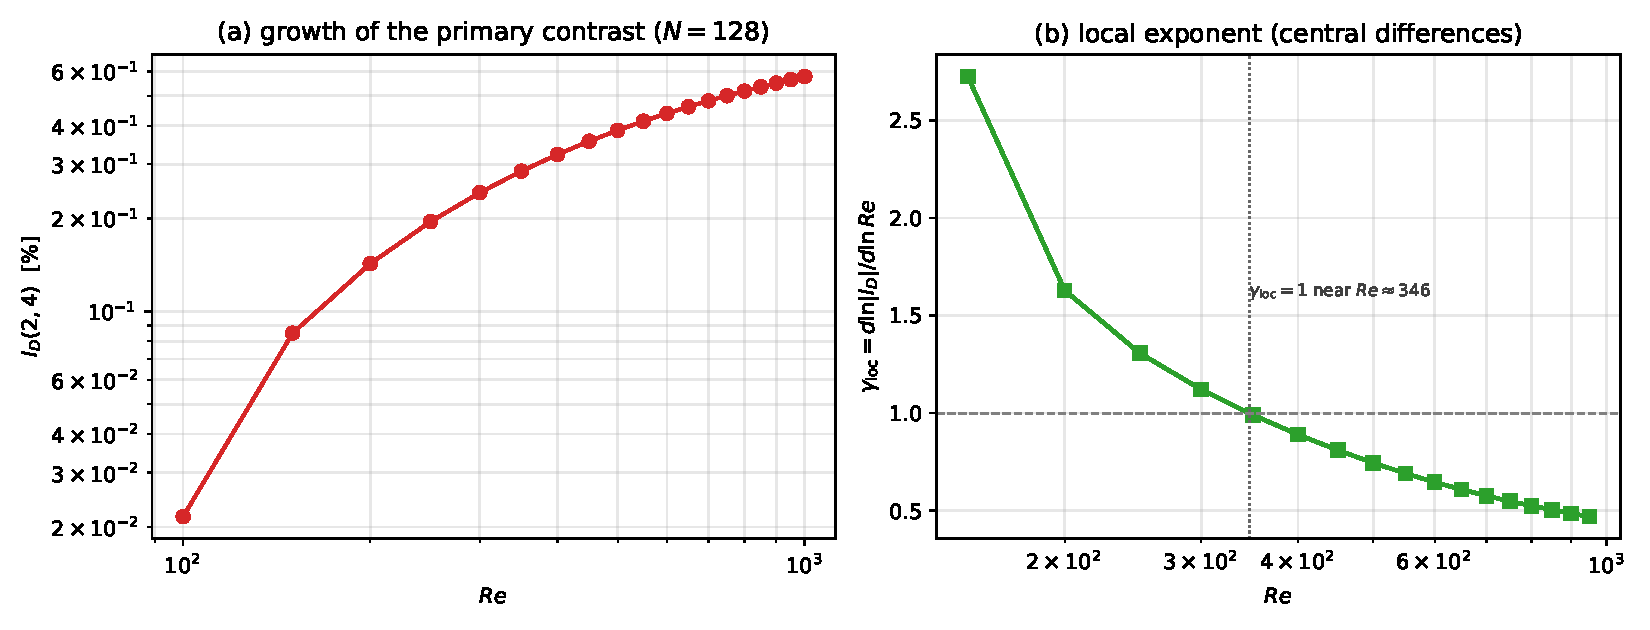
\includegraphics[width=0.98\columnwidth]{figures/fig9_resweep.pdf}
\caption{(Color online) Reynolds-number dependence of the primary contrast $I_D(2,4)$ at $\alpha=0$ from the $N=128$ sweep. (a) log--log growth from $Re=100$ to $1000$. (b) Local exponent $\gamma_{\rm loc}=d\ln|I_D|/d\ln Re$ (central differences), which falls smoothly through unity near $Re\approx346$. The local slope decreases through unity over this exploratory sweep, indicating a transition from superlinear to sublinear growth; these slopes are descriptive and do not establish a universal scaling law.}
\label{fig:resweep}
\end{figure}

\subsection{Robustness of the contrast}
\label{subsec:robustness}

The small magnitude of the contrast makes it essential to show that it is not an artifact of a single numerical choice. We report three independent tests, all at $N=384$ and $\alpha=0$.

\emph{(i) Wall-gradient treatment.} Recomputing the local strain rate with a purely one-sided node-based bottom-wall gradient, instead of the geometric wall-distance correction used in the reference diagnostics, changes $I_D(2,4)$ from $0.0218\%$ to $0.0207\%$ ($Re=100$, a relative change of $5.0\%$), from $0.3249\%$ to $0.3212\%$ ($Re=400$, $1.1\%$), and from $0.5909\%$ to $0.5777\%$ ($Re=1000$, $2.2\%$). The contrast therefore survives the change of wall treatment to within a few percent of its own value; the largest relative sensitivity is at $Re=100$, where the absolute contrast is smallest, while at $Re=400$ and $1000$ the change is $1$--$2\%$.

\emph{(ii) Geometry-dependent effective Reynolds number.} Flattening the bottom changes the flow depth, so the effective Reynolds number felt by the flow differs slightly between the two geometries; an upper bound of $0.4\%$ on this difference (the relative change of the characteristic depth between $n=2$ and $n=4$ times the $Re$ sensitivity) propagates, through the slope $dI_D/dRe$ measured in Section~\ref{subsec:redependence}, to a change of $0.0005\%$ in $I_D(2,4)$ at $Re=100$ (about $2\%$ of its value) and $0.0011\%$ at $Re=400$ (about $0.4\%$). The contrast is dominated by the geometry at fixed $Re$, not by the small $Re_{\rm eff}$ drift.

\emph{(iii) Resolution.} As reported in Section~\ref{subsec:resolution}, $I_D(2,4)$ is stable to within a few percent of its value over the full $N=128$--$384$ range; the absolute integrals are not, and carry a residual grid dependence of order $1\%$. The refinement ratios are not uniform and the residual change between the two finest grids is not a clean power-law decay, so no Richardson extrapolation or grid-convergence index is reported. Instead the observed span of $I_D(2,4)$ over $N=128$--$384$ is retained as the conservative numerical uncertainty: $3.4\times10^{-4}$ percentage points ($Re=100$), $2.4\times10^{-3}$ ($Re=400$), and $1.3\times10^{-2}$ ($Re=1000$), i.e.\ at most $2.3\%$ of the finest-grid contrast. The extrapolated values are not used; the $N=384$ values are quoted throughout, with this span as their resolution uncertainty.

The three tests are mutually consistent and bound the contrast to be robust to wall treatment, to the effective-Reynolds drift, and to resolution, at the level of a few percent of its own value. An independent finite-element (Taylor--Hood) solution was additionally used to cross-validate the LBM bulk solver, both on the benchmark cavity (Section~\ref{subsec:validation}) and, on the superelliptic family, at the level of the primary contrast itself. All finite-element energetics are native (element-wise integrals, no projection), and their energy balance closes to $0.01\%$ on $nx=256$ (and within $0.22\%$ over all meshes, contrasting with the $\approx 2\%$ LBM shear-layer defect). On three meshes ($nx=64/128/256$) the finite-element dissipation contrast is $I_D(2,4)=+0.346\%,+0.332\%,+0.323\%$, and the finest-mesh value $+0.323\%$ lies $0.002$ percentage point from the lattice-Boltzmann value $+0.325\%$ at $N=384$; on the matched finest grids (FEM $nx=256$, LBM $N=384$) all three contrasts agree to within $0.02$ percentage point, and the absolute levels agree to $1$--$4\%$ (Section~\ref{subsec:validation} and the supplementary material). Because the finite-element variation across its own meshes exceeds the final FEM--LBM gap, this is a cross-solver consistency check for the contrast rather than an independent convergence result. A broader cross-solver sweep over the full parameter matrix remains a follow-up.

\subsection{Energetic consistency and estimator agreement}
\label{subsec:consistency}

Two distinct diagnostics are reported. First, the global energy balance of each simulation: the signed relative imbalance $(P^*-D^*)/D^*$ is negative in every case, with magnitude about $2\%$ at $N=384$ ($1.98\%$ at $Re=100$, $2.04\%$ at $Re=400$, $2.13\%$ at $Re=1000$). This residual is not a constant; it decreases with grid refinement as a first-order (in $1/N$) discretisation error, from $-6.2\%$ at $N=128$ to $-2.0\%$ at $N=384$ at $Re=400$ (Section~VII.A of the Supplemental Material). It is therefore a resolution-limited defect of the absolute integrals, not a fixed offset between the lid momentum-exchange estimator of $P$ and the strain-rate estimator of $D$. Second, the agreement between the power-based and dissipation-based estimates of the same matched contrast, $\delta_{IP/ID}=100|I_P/I_D-1|$. For the dominant transition $(2,4)$ at $\alpha=0$, the values are $3.1\%$ ($Re=100$), $1.0\%$ ($Re=400$), and $1.9\%$ ($Re=1000$): the two independent routes to the contrast agree to a few percent at $N=384$.

The agreement degrades for the weaker transitions: at $Re=400$, $\delta_{IP/ID}$ is $10.3\%$ for $(4,6)$ and undefined in any meaningful sense for $(6,8)$, where both $I_P$ and $I_D$ are at the level of $10^{-4}\%$ and their ratio is dominated by cancellation. This degradation is expected: a small difference of two large numbers is sensitive to the small systematic offset between the $P$ and $D$ estimators. It is therefore the dominant $(2,4)$ contrast, not the weak higher-order transitions, that supports a quantitative consistency statement. The reason the contrast is stable even though the absolute defect is not is that, at fixed $(\tau,U)$, the $n = 2$ and $n = 4$ states carry the same leading-order discretization and compressibility defect, which therefore cancels to first order in the paired difference. This is demonstrated, not assumed, by the grid $\times$ Mach factorial of Table~SM.IV: at $Re = 400$ a factor-eight change of $Ma$ moves the absolute defect by $2.0$ points at $N = 128$ (from $-4.24\%$ to $-6.25\%$) but moves $I_D(2,4)$ by only $0.0019$ point, i.e.\ by about $0.6\%$ of its own value. Crucially, this estimator agreement does not replace the resolution analysis: the two estimators may agree well at a given $N$ while both still carry a common grid error. The resolution study of Section~\ref{subsec:resolution} remains the relevant test of grid sensitivity.

\subsection{Influence of the undulation amplitude and integration}
\label{subsec:amplitude}

The amplitude $\alpha$ has two effects. First, it reduces the fluid area at fixed $n$ (by about $5.6\%$ from $\alpha=0$ to $0.1$ at $n=2$) and produces a corresponding uniform downward shift of $P^*$ and $D^*$ (Fig.~\ref{fig:energetic}). Second, and more importantly, it modifies the magnitude of the geometric contrast itself. At $Re=400$ the $(2,4)$ contrast falls from $+0.325\%$ at $\alpha=0$ to $+0.133\%$ at $\alpha=0.1$; at $Re=1000$ it falls from $+0.591\%$ to $+0.078\%$; at $Re=100$ it falls from $+0.022\%$ to $+0.008\%$. This is a genuine interaction in the sense of Section~\ref{subsec:interaction}: the change in the contrast produced by increasing $n$ depends on the undulation amplitude. In percentage points, the interaction for $(2,4)$ at $Re=400$ is $-0.19$, i.e.\ the contrast at $\alpha=0.1$ is about $0.19$ percentage points smaller than at $\alpha=0$. The hierarchy remains qualitatively the same at both amplitudes, but its quantitative strength is amplitude-dependent, and the contrast is weaker when the wall is undulated.

At $Re=1000$ and $\alpha=0.1$ the sign structure itself changes: while $(2,4)$ is still positive at this amplitude ($+0.0782\%$), both $(4,6)$ and $(6,8)$ become negative ($-0.0242\%$ and $-0.0052\%$). The interaction between $n$ and $\alpha$ is therefore not only quantitative (weaker contrast) but also qualitative (sign reversal of the trailing transitions). That reversal is not exclusive to the highest Reynolds number: at $\alpha=0.1$ and $Re=400$ the same two transitions are already negative ($-0.0039\%$ and $-0.0017\%$), each larger in magnitude than its own $N=128$--$384$ span. Undulating the wall thus flips the sign of the trailing transitions at both Reynolds numbers, and increasing $Re$ amplifies the effect; at the flat wall ($\alpha=0$), by contrast, the sign of the $(6,8)$ transition is itself a Reynolds-dependent feature---positive and resolved at $Re=100$ ($+0.00042\%$, $5.2$ times its own span), unresolved at $Re=400$, negative and resolved at $Re=1000$.

Taken together, the three levels of the analysis are coherent. The flow fields change only moderately with geometry; the integrated dissipation changes by a small fraction of a percent despite an area change of several percent; and the contrast hierarchy is stable across Reynolds numbers, resolutions, and amplitudes while its magnitude depends on both $Re$ and $\alpha$. The dominant uncertainty is the residual grid dependence of the absolute integrals (about $1\%$), not the stability of the contrasts themselves.

\subsection{Scope and limitations}
\label{subsec:scope}

The results above establish the robustness of the paired contrasts, not the grid-independence of the absolute integrals. We collect here the limits of the present study. (i) No Richardson extrapolation or grid-convergence index is reported, because the refinement ratios are not uniform and the residual change between the two finest grids is dominated by partial cancellation of common discretisation error rather than by a clean power-law decay; the span of $I_D(2,4)$ over $N=128$--$512$ is retained as the conservative numerical uncertainty. (ii) The absolute integrals carry a residual grid dependence of order $1\%$ between $N=256$ and $N=384$; no claim of grid-independent absolute energetics is made. (iii) The Taylor--Hood finite-element comparison is a cross-solver consistency check, not a convergence proof for either solver, because the finite-element variation across its own meshes exceeds the FEM--LBM gap. (iv) The scope is limited to the tested superellipse family, single undulation count $N_w=1$, and the three Reynolds numbers studied; the unmatched Mach numbers of the coarse $n\ge6$ runs at $Re=100$ preclude any claim that the trailing-transition signs at $Re=100$ are grid-converged. (v) The $N=512$ extension is available only at $Re=400$ and $Re=1000$, $\alpha=0$; it confirms the stability of the primary contrast (to within $3\times10^{-5}$~pp between $N=384$ and $N=512$ at $Re=400$) and strengthens the negative sign of the $(6,8)$ transition at $Re=1000$, but does not alter the qualitative conclusions drawn from the $N=128$--$384$ sequence.

Table~\ref{tab:claims_evidence} collects the main claims of this study, the evidence on which each rests, and the associated uncertainty. The purpose is to make explicit which conclusions are resolution-backed and which remain qualitative or partial.

\begin{table*}[!htbp]
\centering
\caption{Summary of claims, evidence, and uncertainties. Each row pairs a central statement with the data that support it and the resolution or modeling limitation that bounds its interpretation. ``Resolved'' indicates whether the claim is backed by a contrast whose magnitude exceeds its own $N=128$--$512$ span.}
\label{tab:claims_evidence}
\resizebox{\textwidth}{!}{%
\begin{tabular}{@{}llll@{}}
\hline
\textbf{Claim} & \textbf{Evidence} & \textbf{Uncertainty} & \textbf{Resolved?} \\
\hline
$I_D(2,4)>0$ at $Re=100,400,1000$ & $N=384$ values; spans & $3.4\times10^{-4}$, $2.4\times10^{-3}$, $1.4\times10^{-2}$~pp & Yes \\
Hierarchy $|I(2,4)|\gg|I(4,6)|\gg|I(6,8)|$ & $N=384$ + per-transition spans & Own spans per transition & Yes at $Re=400,1000$; partial at $Re=100$ \\
$\mathrm{d}B>0$ at all $Re$ & four bands at $N=128$--$512$ (Table~SM.XV) & positive on every grid; magnitude $\le3\%$ span & Yes (sign) \\
$\mathrm{d}A$ changes sign near $Re\approx145$ & four bands at $N=128$--$512$ (Table~SM.XV) & sign stable across grids; magnitude up to $27\%$ at $Re=1000$ & Yes (sign) \\
Sub-extensivity (factor 13--364) & $I_D$ vs $I_{D,\text{area}}$ & Dominated by $I_D$ uncertainty & Yes \\
FEM--LBM cross-solver consistency & $nx=256$ vs $N=384$ & 0.002--0.008~pp & Consistency only \\
\hline
\end{tabular}%
}
\end{table*}










\section{Conclusions}
\label{sec:conclusions}

This study examines the energetic response of a lid-driven cavity to superelliptic bottom-wall shaping. For $n=2\to4$ at $\alpha=0$, fluid area increases by $7.93\%$, but integrated dissipation rises by only $0.0218\%$, $0.3249\%$, and $0.5909\%$ at $Re=100$, $400$, and $1000$. An area-only reference overpredicts these contrasts by factors of $364$, $24$, and $13$. Dissipation per unit fluid area decreases by about $7\%$, showing that area change alone cannot explain the response.

An exact spatial partition separates dissipation in the newly opened shoulder region from redistribution over the region common to both geometries. This $\mathrm{d}A/\mathrm{d}B$ decomposition, which constitutes the central original contribution of the present work, provides direct physical insight into the mechanism underlying the sub-extensive response: at $Re=400$, the added region occupies $7.4\%$ of the fluid area but contributes only $0.2\%$ of the reference dissipation, while the common-region redistribution is itself a near-cancellation of opposing lid-band and core-band contributions. The common-region contribution is negative at $Re=100$ and positive at $Re=400$ and $1000$, reflecting a Reynolds-dependent balance between near-wall and core changes. The net contrast remains positive throughout. The grid robustness of this mechanism is assessed in Table~SM.XV and Fig.~SM.5: all four bands are recomputed with the same exact-partition code at every resolution $N=128$--$512$; the cancellation index $C=\sum|\text{bands}|/|\mathrm{d}A|$ grows from $4.0$ at $Re=100$ to $14.3$ at $Re=1000$, but the net contrast $\Delta D=\mathrm{d}A+\mathrm{d}B$ remains stable to within $2.4\%$ across all grids because the grid-induced changes in $\mathrm{d}A$ and $\mathrm{d}B$ partially cancel. The sign and order of magnitude of $\mathrm{d}A$ and $\mathrm{d}B$ are therefore robust on every grid; their individual magnitudes carry a grid sensitivity that rises with $Re$ (the $\mathrm{d}A$ span is $1.9\%$, $8.2\%$ and $27\%$ of its value at $Re=100$, $400$ and $1000$). At $Re=100$, the energy-balance defect varies by $3.8$ points between $N=128$ and $N=384$ while $I_D(2,4)$ remains within $3.4\times10^{-4}$~pp (Table~SM.XIX), confirming that the defect is a common-mode error that cancels in the paired contrast.

The response is concentrated in the $n=2\to4$ transition at all Reynolds numbers studied, which carries about $96.2\%$ of the summed absolute contrasts at $Re=400$. The full exponent sequence is now available at all three Reynolds numbers: at $\alpha=0$ the $n=4\to6$ contrast is $+0.00296\%$, $+0.0129\%$, and $+0.0103\%$, and the $n=6\to8$ contrast is $+0.00042\%$, $+6\times10^{-5}\%$, and $-0.0037\%$ at $Re=100$, $400$, and $1000$. Resolution is judged transition by transition against each contrast's own $N=128$--$384$ span. At $Re=1000$ both trailing steps are resolved, the $(6,8)$ step by a factor of $34$ and with the same negative sign on all three grids, so it is reported as the first resolved negative trailing step. At $Re=400$ that step lies inside its own span, so its sign is undetermined; at $Re=100$ the $(4,6)$ step cannot be resolution-tested, because its two coarser members mix Mach regimes, and it too is quoted as an upper bound. At $\alpha=0.1$ the two trailing transitions are negative and individually resolved at both $Re=400$ and $Re=1000$, so wall undulation fixes their sign already at moderate Reynolds number. Increasing undulation amplitude also weakens the primary contrast. Across $N=128$, $256$, and $384$, the primary $\alpha=0$ contrast varies by at most $2.3\%$ of its own value, although absolute integrals retain about $1\%$ grid sensitivity. Independent Taylor--Hood finite-element calculations reproduce the primary contrast to $0.002$ percentage points at $Re=400$ and to $0.008$ percentage points at $Re=1000$, on the finest meshes of each solver. Scope is limited to the tested superellipse family and single undulation count; the unmatched Mach numbers of the coarse $n\ge6$ runs at $Re=100$, together with residual grid sensitivity, preclude universal scaling or grid-independent claims. Numerical uncertainties on $I_D(2,4)$ are $3.4\times10^{-4}$, $2.4\times10^{-3}$, and $1.4\times10^{-2}$ percentage points at $Re=100$, $400$, and $1000$; the trailing contrasts have their own, generally smaller spans, collected in Table~SM.X, and are $6.9\times10^{-4}$ and $1.1\times10^{-4}$ percentage points at $Re=1000$, well below the corresponding magnitudes.


\section*{Supplementary Material}
The supplementary material contains the following items, referenced throughout the main text as Table~SM.I--SM.XIX, Fig.~SM.1--SM.6, and Section~VII.F:
\begin{itemize}
\item Geometry function, parameter ranges, and fluid areas (Table~SM.I);
\item Full LBM numerical parameter set for the production and test grids (Table~SM.II);
\item Reynolds-sweep LBM parameters at $N=128$ (Table~SM.III);
\item Grid$\times$Mach factorial design (Table~SM.IV);
\item Exact square-cavity verification against Ghia et al.\ centerline profiles, including the near-square ($n=8$) case (Table~SM.V);
\item Regularized-lid isolation test: complete $Re\times N\times\{$uniform, regularized$\}$ matrix (Table~SM.VI);
\item Independent Taylor--Hood finite-element method (FEM) cross-validation: native mesh convergence and FEM--LBM contrast comparison at $Re=400$ and $Re=1000$ (Tables~SM.VII and SM.VIII);
\item Complete energetic dataset ($P^*$, $D^*$, $K^*$, $A_f$) for all 24 configurations at $N=384$ (Table~SM.IX);
\item Full contrast dataset ($I_D$, $I_P$, $\delta_{IP/ID}$, spans) for all resolutions $N=128$--$512$, transitions, and amplitudes (Table~SM.X);
\item Energy-balance audit $\varepsilon_E = |P^*-D^*|/D^*$ at $N=384$ for all configurations (Table~SM.XI);
\item Energy-balance audit at the $N=512$ extension ($Re=400$ and $1000$, $\alpha=0$) (Table~SM.XII);
\item Flow-field maps (velocity magnitude and streamlines) for every converged configuration, separated by amplitude (Figs.~SM.2 and SM.3);
\item Resolution-dependence figure for $I_D(2,4)$ and $\delta_{IP/ID}$ (Fig.~SM.4);
\item Exact spatial decomposition of the dissipation contrast into $\mathrm{d}A$ (four-band common region) and $\mathrm{d}B$ (added region) at $N=384$ (Table~SM.XIII and Fig.~SM.6);
\item Partition $\mathrm{d}A$, $\mathrm{d}B$ along the $N=128$ Reynolds sweep (Table~SM.XIV);
\item Grid robustness of the $\mathrm{d}A/\mathrm{d}B$ partition, with all four bands recomputed at every resolution $N=128$--$512$ and the cancellation index, plus its resolution-dependence figure (Table~SM.XV and Fig.~SM.5);
\item Exploratory Reynolds sweep: primary contrast $I_D(2,4)$ and local exponent $\gamma_{\mathrm{loc}}$ (Table~SM.XVI);
\item Area-reference comparison: measured $I_D$ vs.\ area-only prediction $I_{D,\mathrm{area}}$ (Table~SM.XVII);
\item Amplitude-interaction table: $I_D(2,4)$ at $\alpha=0$ and $\alpha=0.1$ (Table~SM.XVIII);
\item Re=100 energy-balance defect versus the paired contrast, showing common-mode cancellation (Table~SM.XIX);
\item Robustness tests: wall-gradient treatment, effective-Reynolds perturbation, and discrete-vs-analytic area comparison (Section~VII.F).
\end{itemize}

\begin{acknowledgments}
\par\vspace{0.5ex}
This work was carried out at the Laboratory of Fluid Mechanics, Ecole Militaire Polytechnique, Algiers, Algeria. No external funding was received.
\end{acknowledgments}

\section*{Author Declarations}
\subsection*{Conflict of Interest}
The author declares no conflict of interest.
\subsection*{Author Contributions}
A.~Beniaiche: Conceptualization, Methodology, Software, Investigation, Formal analysis, Validation, Writing -- original draft, Writing -- review \& editing.

\section*{Data Availability Statement}
The data that support the findings of this study are available within the article and its supplementary material. The converged scalar datasets, velocity-field arrays, and post-processing scripts that support the findings of this study are available from the corresponding author upon reasonable request.

\bibliography{references}

\end{document}
